\documentclass[conference]{IEEEtran}
\IEEEoverridecommandlockouts
% The preceding line is only needed to identify funding in the first footnote. If that is unneeded, please comment it out.
\usepackage{cite}
\usepackage{amsmath,amssymb,amsfonts}
\usepackage{algorithmic}
\usepackage{graphicx}
\usepackage[inline]{enumitem} 
\usepackage{textcomp}
\usepackage[]{algorithm2e}
\usepackage{xcolor}
\usepackage[hyphens,spaces,obeyspaces]{url}
\usepackage{multirow}
\usepackage{amsmath}
\definecolor{LightGray}{gray}{0.9}
%%personal macros --begin%%
%%%%%%%%Useful macros for poof-reading, always copy-paste into your latex projects
\usepackage[colorinlistoftodos,prependcaption,textsize=tiny]{todonotes}
\usepackage{listings}
\usepackage{minted}

\newboolean{showcomments}
\setboolean{showcomments}{true} % toggle to show or hide comments
\ifthenelse{\boolean{showcomments}}
{\newcommand{\nb}[2]{
		\fcolorbox{black}{yellow}{\bfseries\sffamily\scriptsize#1}
		{\sf\small$\blacktriangleright$\textit{#2}$\blacktriangleleft$}
	}
	\newcommand{\version}{\emph{\scriptsize$-$working$-$}}
}
{\newcommand{\nb}[2]{}
	\newcommand{\version}{}
}
\newcommand\patrizio[1]{\nb{Patrizio}{#1}}
\newcommand\sergio[1]{\nb{Sergio}{#1}}
\newcommand\tb[1]{\nb{Thorsten}{#1}}

% Macros for proof-reading
\usepackage[normalem]{ulem} % for \sout
\usepackage{xcolor}
\usepackage{array}
\usepackage{booktabs}
\usepackage{scalerel}
\usepackage[para,online,flushleft]{threeparttable}
\usepackage{booktabs}
\usepackage{pifont}
\newcommand*\rot{\rotatebox{90}}
\newcommand*\OK{\ding{51}}
\newcommand{\xmark}{\ding{55}}%
\newcolumntype{P}[1]{>{\centering\arraybackslash}p{#1}}
\newcommand{\ra}{$\rightarrow$}
\newcommand{\ugh}[1]{\textcolor{red}{\uwave{#1}}} % please rephrase
\newcommand{\ins}[1]{\textcolor{blue}{\uline{#1}}} % please insert
\newcommand{\del}[1]{\textcolor{red}{\sout{#1}}} % please delete
\newcommand{\chg}[2]{\textcolor{red}{\sout{#1}}{\ra}\textcolor{blue}{\uline{#2}}} % please change
%%%%%%%%
%Macros
% Footnotes
\newcommand{\foot}[1]{\footnote{\url{#1}}}
%%personal macros --end%%
\def\BibTeX{{\rm B\kern-.05em{\sc i\kern-.025em b}\kern-.08em
    T\kern-.1667em\lower.7ex\hbox{E}\kern-.125emX}}

\begin{document}

\title{MoTiVML: A Flexible and Customizable Variability Modelling Language for Robotic System Design\\
%{\footnotesize \textsuperscript{*}Note: Sub-titles are not captured in Xplore and
%should not be used}
%\thanks{Identify applicable funding agency here. If none, delete this.}
}

\author{\IEEEauthorblockN{Jude Gyimah}
\IEEEauthorblockA{\textit{Department of Computer Science and Engineering} \\
\textit{Chalmers $|$ University of Gothenburg}\\
Gothenburg, Sweden \\
gusgyiju@student.gu.se}
\and
\IEEEauthorblockN{Sergio Garc\'{i}a}
\IEEEauthorblockA{\textit{Department of Computer Science and Engineering} \\
\textit{Chalmers $|$ University of Gothenburg}\\
Gothenburg, Sweden \\
sergio.garcia@gu.se}
\and
\IEEEauthorblockN{Thorsten Berger}
\IEEEauthorblockA{\textit{Department of Computer Science and Engineering} \\
\textit{Chalmers $|$ University of Gothenburg}\\
Gothenburg, Sweden \\
thorsten.berger@chalmers.se}
\and
\IEEEauthorblockN{Patrizio Pelliccione}
\IEEEauthorblockA{\textit{Department of Computer Science and Engineering} \\
\textit{Chalmers $|$ University of Gothenburg}\\
Gothenburg, Sweden \\
patrizio.pelliccione@gu.se}
}

\maketitle

\begin{abstract}
Technological advancements have led to a growing demand for efficient solutions that minimise risk and maximise efficiency when it comes to performing tasks in non-deterministic environments. 
In the wake of the current pandemic, the industrial domain has faced many challenges such as labor and product shortages, logistic limitations, as well as an unexpected strain on human driven supply systems, all due to the enforcement of safety regulations and health complications. Undeniably, these challenges have had a resounding effect across the global service industry; hence the emergence of viable alternatives to alleviate some these problems. One such alternative which is not only feasible but also useful in practice, is the use of service robots.
Service robots are a category of robots that render services to humans. Service robots are often designed to operate in highly heterogeneous environments in collaboration with humans, or other robots. The effective completion of tasks by service robots may require a combination of specific sets of robotic capabilities. These capabilities are mainly driven by robotic features.

Valid combinations of robotic features to fit varying contexts, give rise to some level of variability---i.e., the ability of a software artifact to be changed to fit different contexts, environments, or purposes. This constitutes a possible strategy to enable robotic applications to be adapted, customized, or configured to fit different scenarios. Hence, the need to have an effective mechanism for planning, designing, and implementing variability.

Cognisant of this need, we present a novel technique that implements variation points with reference to feature binding time and binding mode. This implementation comes as an extension of the Self-adaptive dEcentralized Robotic Architecture (SERA) framework architecture. SERA, which is a decentralized architecture that supports the building of autonomous, heterogeneous, and collaborative robotic applications, lacks the ability to manage variability dynamically. For that matter, SERA and its ilk typically do not provide roboticists with the means and techniques required to manage variability effectively.

In our novel approach to solving this problem, we define example systems as feature models, study the variability of these feature models, and then proceed to conceive a variability-modelling language, that provides mechanisms for managing variability with respect to binding time and mode. Our solution is offered as an open-source library that provides basic support for binding features in robotic systems.

This study provides evidence of the extensibility of robotics reference architectures to support variability in a domain where variability is typically performed in an ad hoc manner. For that matter, our solution is expected to alleviate extension complexities, reduce performance costs, and minimize resource consumption in robotic systems while giving roboticists the flexibility boost they so desire when it comes to engineering robotic systems.

Furthermore, through the design science approach, this conclusive study provides evidence to back the claims that our proposed variability management technique is novel, realizable and useful in practice. Along with a means for assessing model configuration validity.
\end{abstract}

\begin{IEEEkeywords}
variability modelling, service robots, robotics software engineering, domain specific languages, feature reconfiguration, flexible feature binding
\end{IEEEkeywords}

\section{Introduction}
\label{section:intro}
%%general intro --start%%
Service robots---``{\em a type of robot that performs useful tasks for humans or equipment excluding industrial automation applications}'' \foot{https://www.iso.org/standard/55890.html}---are gradually becoming an integral part of human existence. It is estimated that the service robotics industry will be valued at 24 billion US dollars by the year 2022.\foot{https://www.marketsandmarkets.com/Market-Reports/ivd-bric-market-198.html}
According to the International Service Robot Association, service robots can be classified as machines that sense, think, and act to benefit or extend human capabilities and to increase human productivity \cite{serv-rob-his}. This implies service robots are sometimes conceived, built, and used as intermediate solutions to assist humans in performing daunting and repetitive tasks.

As cyber-physical systems, service robots are often designed to operate in highly heterogeneous environments in collaboration with either humans, other robots, or both. Practical implementations of such service robots include UVD's Model C \foot{https://www.uvd-robots.com} and PAL Robotics's TIAGo Base\foot{http://blog.pal-robotics.com/how-to-build-a-solution-for-fighting-coronavirus-using-the-tiago-base-robot/} 
disinfection range of robots, which have been deployed in the fight against the spread of COVID-19, in areas such as shopping centers, airports, and hospitals across the globe.

In any given context of operation, a robot only needs a defined subset of core assets, otherwise referred to as features, that define the robot's capabilities. A feature can be classified as a logical unit of behavior defined by a set of functional and non-functional requirements \cite{feats}. Depending on the usage context, features may be selected or deselected as part of a configuration to drive a given set of capabilities. 

For example UVD's disinfection range of robots, operate by moving at a sufficient speed in a 360-degree fashion, while emitting enough UV-C ultraviolet light on relevant surfaces to eliminate viruses and bacteria. In doing so the UVD robot may make use of core assets such as navigation, obstacle detection, collision avoidance, disinfection, and teleoperation appropriately.

Valid combinations of these core assets to match the operation of the robot in a given context gives rise to some level of variability in the robotic system. By definition, variability can be described as the ability of a core asset to adapt to usage in different product contexts that are within a product line scope \cite{variab}. The goal of managing variability is to create cost-effective and customisable core assets that are easy to build.

All decisions on variability in design have to be communicated and documented for future use. As an important consequence, it is necessary to have clear representations for variation points, variants, and mechanisms to realise variability. These said representations of product lines can be depicted using a reference architecture.

A reference architecture which is essentially a predefined architectural pattern, or set of patterns, captures the high-level design for the applications of a software product line \cite{sple}. These patterns could be partially or completely instantiated, designed and proven for use in specific business and technical contexts, together with supporting artifacts \cite{ref-arch}.

In this study, we focus on the Self-adaptive dEcentralized Robotic Architecture (SERA) \cite{sera}. As an architecture for decentralized, collaborative, and autonomous robots, SERA was conceptualized and designed to support human-robot collaboration, as well as adaptation and coordination of single and multi-robot systems in a decentralized fashion.

The SERA architecture and its ilk do not typically support any standardised form of variability management. This is, however, not desirable in a complex yet innovative domain such as robotics. Robots are mandated to operate in a variety of environments, which are often unpredictable and human-populated. To operate in such heterogeneous environments, robots possess many different capabilities in the form of functional and non-functional characteristics, which are reusable in variable environmental contexts.

In this study, we extend the capabilities of the SERA architecture to include variability management, with a high level of flexibility and customizability of robotic product line entities, while improving practices currently present in the robotics applications development domain.

This is particularly useful because, just like SERA, most known architectures of that nature, manage variability using ad hoc mechanisms. These architectures often do not provide any means of controlling product entity bindings in a systematic way. Such reference architectures are also incapable of tracking and providing an overview of product entity commonalities and variabilities together with their dependencies consistently \cite{var-mod-ind}.

One of the fundamental concepts of adaptable software architectures is their ability to establish an overview of understanding, by systematically modeling the adaptation space using representations such as feature models, while having dedicated techniques to match such adaptations.

In this study, our overall goal is to provide roboticists with a variability modelling language that has the means and techniques for planning, designing, and implementing variability. We achieve this by implementing techniques that realize variability. These techniques, typically referred to as variability mechanisms, comprise of a means for modelling variability such as feature models, and techniques that implement variation points within the feature models. \cite{var-mod-ind}.

This study, contributes a novel technique for implementing variation points in robotic systems via a feature's binding time and binding mode. Time and mode bindings are implemented as an extension to feature models \cite{flex-feat-bind}, where binding time is defined as either compile time or runtime, while binding mode is defined as either static or dynamic. Usually, the semantics of such an implementation can be potentially complex, since valid feature reconfigurations are not only constrained by dependencies, but also by valid/invalid combinations of bindings that exist between dependent features.

In summary, our work provides a variability modelling language, in response to the following domain challenges:
\begin{enumerate}
    \item \textit{The lack of a standardised variability modelling language: }The lack of a standardised variability modelling language for managing features centrally, modeling features together with their possible bindings and assuring model correctness with valid configurations. Various ad hoc mechanisms exist, but no standardized solution exists on how to manage variability within the robotics domain. For example in ROS, dynamic features can be realized using parameterization\foot{http://wiki.ros.org/Parameter\%20Server} or loadable ROS plugins.\foot{http://wiki.ros.org/pluginlib} Static features on the other hand, might need a preprocessor and some inclusion into the build system.
    
    \item \textit{The lack of guidelines for implementing variability management techniques in robotic systems:} Even though a plethora of techniques exist, there are no specific guidelines that detail which technique to use and how to use it within the robotics domain.
    
    To the best of our knowledge, open sourced ROS based applications lack some form of a comprehensive documentation in the form of usage guidelines that verify or provide proof that such robotic applications meet the specifications or requirements that define their capabilities.
    
    \item \textit{The lack of a variability management solution that addresses the complexity of engineering robotic systems: }A full-fledged robotic system is a complex system that consists of many modules. Whether single purpose or multi purpose, the versatility a robotic system offers in different scenarios, requires the integration of heterogeneous modules. Many of these modules that need to be integrated are developed by a diverse group of experts (e.g., electrical engineers, perception experts, control theorists, software engineers). This perceivable diversity complicates the integration, customisation, and maintainability of packages in robotic systems. These complications translate into complexity when it comes to engineering robotic applications.
\end{enumerate}

In realising a solution such as ours, a key requirement was to keep it as lightweight as possible without requiring new tooling; all the while maintaining a decent level of abstraction. Thus, we relied on the design science approach which was empirically guided by the following research questions.
\begin{itemize}
     \item \textbf{RQ 1: }\emph{What are example instances of feature realizations with different binding modes and binding times in a ROS-based robotic system?}
     
     Example instances of feature realisations can be derived from example systems of service robots. Depending on their operational domain, these example systems may possess different sets of features that can be bound at different times and modes.
    
    \item \textbf{RQ 2: } \emph{How can a variability modelling language that allows modelling features together with their binding times and binding modes be designed?}
    
    A variability modelling language that allows modeling features together with their binding times and binding modes can be designed by first of all clarifying the key relevant aspects of the language domain, through domain analysis. Based on that the abstract syntax, concrete syntax and static semantics of the language can be derived.
    
    \item \textbf{RQ 3:} \emph{What mechanisms and guidelines can be used to implement features with the different binding times and modes in a ROS-based robotic system?}
    
    Variability mechanisms are implementation techniques to realize variability. In our variability modelling language, we provide formalisms for modelling features based on the variant derivation concepts of feature models as well as a novel variation mechanism based on feature binding time and binding mode. We also provide guidelines for the above stated variability mechanisms in the form of a concise documentation to assist domain stakeholders in implementing custom models of their own.
\end{itemize}
%% Research Questions --end%%

\section{Literature Review}
Determining valid feature configurations based on features'  binding time and mode can be tricky and somehow cumbersome. For this reason, there needs to be an optimum mechanism for deriving configurations that alleviates some of these complexities. As an antecedent of such an optimum mechanism, the dependencies and constraints that exist between features must be well established.

A vast variety of key studies in the domain of robotic applications development, architecture design and variability management served as inspiration to this study. The most prominent of these being SERA. SERA as a layered architecture that contains components that manage robotic system adaptations at different levels of abstraction was conceived by Garc\'{i}a et al. \cite{sera} to solve three distinct problems, namely:
\begin{enumerate*}[label=(\roman*)]
	\item the lack of architectural models and methods in the production of software for robotic systems,
	\item the absence of a common approach or strategy that might allow vendors to produce their own robots and deploy them within a team, and
	\item the lack of systematic support for adaptations of robot teams.
\end{enumerate*}

By communicating through well-defined interfaces, SERA has the ability to be implemented within a wide variety of projects. SERA's architecture can be realized using different middlewares and component frameworks related to robotics. This further emphasises the extensibility of its framework architecture in anticipation of future changes.
That notwithstanding, SERA and architectures similar to it, lack adaptation capabilities. More so as an architecture for collaborative and autonomous systems, runtime adaptation in particular remains a top priority in SERA's operation due to the level of adaptation complexity that exists in the domain of collaborative autonomous systems. To deliver this, we have implemented an extension to the SERA's architecture, in the form of an open source library, that offers a domain specific language(DSL) implemented in Python\foot{https://www.python.org/} and C++\foot{https://isocpp.org/}.

\subsection{Domain-Specific Languages}
\textit{``A domain-specific language (DSL) is a programming language or executable specification language that offers, through appropriate notations and abstractions, expressive power focused on, and usually restricted to, a particular problem domain''} \cite{dsl}.

Domain-Specific Languages (DSLs) are usually declarative. One of the key characteristic of DSLs is their focus on expressive power. They allow solutions to be expressed at the level of abstraction of the problem domain. For this reason, domain experts can understand, validate, modify, and often even develop DSL programs \cite{dsl}.

Developing advanced robotic systems can be challenging as expertise from multiple domains need to be integrated conceptually and technically. Through domain-specific modeling, robotic concepts and notations can be modelled descriptively. This raises the level of abstraction and results in models that are easier to understand and validate. Furthermore, DSLs increase the level of automation, e.g., through code generation, while bridging the gap between modeling and implementation \cite{dsl-robo}. Besides automation of software development through code generation, there are several added benefits of DSLs. These include analysis, optimization, and most importantly the inclusion of non-developer stakeholders into the process of software creation.

Literally hundreds of DSLs are in existence. Of these, only a subset of them are described in software engineering or programming language literature. Best-known classical examples are PIC, SCATTER, CHEM, LEX, YACC, Make, KRL\foot{https://pdfcoffee.com/kss-55-operating-and-programming-instructions-for-end-userspdf-pdf-free.html} and MARTe.

Inspirational concepts for our language were drawn from existing DSLs, so as to offer a user friendly yet intuitive language that possesses an optimum level of abstraction that fits the needs of multiple end users with varying skill sets. With dsl zoo \cite{dsl-robo} as a reference point, annotated bibliographies of domain-specific languages in the area of robotics and automation technology were carefully studied. Example DSLs in that capacity include Mauve\foot{https://corlab.github.io/dslzoo/architectures-and-programming-subdomain.html#lesire2012mauve}, Robotml\foot{*#dhouib2012robotml}, LE\foot{*#gordillo1991high}, and eTaSL/eTC,\foot{*#aertbelien2014etasl} 

\subsection{Runtime Adaptation}
Run-time adaptation in modern day systems often involves some level of uncertainty. In modern software systems, handling uncertainty in advance is often not feasible and resource intensive. This implies that there may be the need to deal with uncertainty when the knowledge required becomes available. At run-time, robots need to manage huge amounts of different execution variants that can never be foreseen and completely pre-programmed and can thus not be analysed and checked entirely at compile time.

For this reason, Hochgeschwender et al. \cite{graph-mde} employed a model-driven approach. Their approach involves capturing domain knowledge explicitly in the form of domain models. The models which are described by domain-specific languages are needed to be somehow accessed by robots at runtime to take decisions for adaptation purposes. Granting robots access to the software-related models at runtime implies persistently storing the different notations and formats of DSLs, composing the various domain models, and querying over multiple domains at run time. Portions of the methods employed in the study to achieve adaptation align with our study in that resources relevant to the operation of a given robot are modeled using DSLs and stored. The stored models are accessed on demand at runtime, when binding information is available, for the sake of adapting the system to the changing environmental conditions.

As mentioned previously, models are fundamental to the functioning of robots. Steck et al. \cite{model-centric} in their study provide in-depth insight into why models and a model-centric approach to robotics software design and implementation is important.
In their study, they reaffirmed the role in which models provide a means to check the validity of desired configurations and parameterizations of robotic system components. A model-driven approach also feeds into the idea of making an implementation generic enough to be used by multiple platforms. This supports our choice to use feature models as a layer of abstraction over robotic components, where features can be bound with respect to time and mode, to realise runtime adaptation through the runtime reconfiguration of binding units extracted from valid combinations of features.

 In our implementation, valid combinations are determined based on binding time and mode pairs attached to a given set of user selected features. Similarly, Pinto et al. \cite{cont-aware} in the implementation of their middleware framework for context-aware applications, designed the framework to keep a record of policies that are fed with contextual information obtained by an agent (e.g., a robot) interacting with the environment. Actions tied to functions are triggered when the conditions surrounding a policy are satisfied. The policy set is dynamic in that it is updated in real time according the environmental changes experienced by the navigating agent.
 
 This train of thought aligns with design decisions made in the implementation of our framework where robotic features are assigned a specific binding mode and time by the user of the framework and this serves as the underlying policy with which the robot will determine how adaptive it can be with respect to the unloading and loading a feature.
 
\subsection{Managing Adaptation Complexity}
Adaptive systems can be defined as systems that exercise variability to cope with changing system requirements. Adaptive systems support feature binding at runtime and are sometimes called dynamic Software Product Lines (DSPLs). DSPLs are usually built from coarse-grained components, which reduces the number of possible application scenarios. 

As an extension of their previous studies on dynamic feature binding, Rosenmuller et al. \cite{tailor-spl}  conceptualised a feature-based adaptation mechanism that reduces the effort of computing an optimal configuration at runtime. 

To do this effectively, they generate a DSPL from an SPL by statically selecting the features required for dynamic binding and generating a set of dynamic
binding units. To be able to effectively support runtime adaptation of programs, they use a customizable framework, called FeatureAce\foot{https://sourceforge.net/projects/featurecpp/}. By including FeatureAce into a generated DSPL, they are able to compose features and modifying configurations at runtime.

Learning points from this study share similar characteristics to our own study in many ways. First off, Rosenmuller et al\cite{tailor-spl} acknowledge the complexity that exists in software product lines and as such understand that variability can only be manage with an effective mechanism that can keep up with changing requirements, without having to deal with an overwhelming amount of overhead.

 To remedy this problem they chose to use DSPLs composed out of SPLs that are combined into dynamic binding units which can be adapted at runtime. However, we decided to form variability mechanisms using binding time and binding mode as a means of adapting our configurations. The major difference here lies in the fact that our methods are novel and not so much focused on the quality of dynamic binding units. Rather we focus on the feasibility of the mechanism in practice.
 
 \subsection{Feature-Modeling Languages}
With the current set of feature-modeling languages that
are available, Clafer,\foot{https://www.clafer.org/} Kconfig,\foot{https://www.kernel.org/doc/html/latest/kbuild/kconfig-language.html} and CDL\foot{http://www.cse.chalmers.se/~bergert/paper/cdl_semantics.pdf} appear to be quite popular amongst professionals in industry. Clafer is one of the most expressive feature modeling languages that unifies feature and class modeling. The notion of a feature and that of a class is unified into Clafer. Clafer offers types, constraints, and attributes. Clafer supports multi-level modeling and has well-specified semantics as well as rich tooling, including instance generation, configuration, and visualization. As a textual language, it has one of the simplest, expressive and most intuitive syntax out there today \cite{fmod-lang-scenarios}. The language is built on top of first order logic with quantifiers over basic entities combined with linear temporal logic \cite{clafer}.

\textit{Kconfig} and \textit{CDL} are languages that have the capability to describe the variability of systems. Even though \textit{Kconfig} and \textit{CDL} share similar concepts, they were developed independently from each other, and independently from feature modeling languages with research origin \cite{vmir}. Kconfig and CDL are two of the most successful languages, primarily used in the systems software domain \cite{fmod-lang-scenarios}. 

In a study conducted by Berger et al. \cite{fmod-lang-scenarios}, a feature modeling language that is intuitive, simple, and also expressive enough to cover a range of important usage scenarios must make provision for a base set of usage scenarios namely Exchange, Storage, Domain Modeling, Teaching and Learning, Mapping to implementation, Model generation, Benchmarking, and Analyses. These selected scenarios were derived from a large number of general usage scenarios elicited from researchers at a meeting during the Software Product Line Conference (SPLC) in September 2018 in Gothenburg.

Despite the fact that most of these languages share concepts, they also present several limitations. These perceivable limitations have influenced our decision to propose yet another feature modelling language. In comparison to the others, our proposed language has been evaluated based on five characteristic properties. These characteristics properties confirm the relevance and novelty of our feature-modelling language with respect to others, in the robotics domain. The five characteristic properties include:
\begin{enumerate*}[label=(\roman*)]
	\item C1: Expressiveness
	\item C2: Covers a wide range of usage scenarios
	\item C3: ROS compatible
	\item C4: Can describe variability
	\item C5: Abstract syntax supports variability modelling based on binding time and binding mode
	\item C6: Enforces and evaluates modelling constraints.
	\item C7: Implements binding time and binding mode as a variation mechanism.
	\item C8: Provides implementation guidelines and mechanisms.
\end{enumerate*}

Table \ref{tab:compfml} shows how our proposed feature modelling language compares to other languages with respect to our chosen characteristics.
\begin{table}[htbp]
\caption{Characteristic Comparison of Feature-Modelling Languages}
\begin{center}
\begin{tabular}{|c|c|c|c|c|c|c|c|c|}
\hline
    Language & C1 & C2 & C3 & C4 & C5 & C6 & C7 & C8 \\ \hline
    PyFML & $\bullet$ & $\bullet$ &  &  & & $\bullet$ & &\\\hline
    HyperFlex & $\bullet$ & $\bullet$ & $\bullet$ & $\bullet$ &  & $\bullet$ & &\\\hline
    TVL & $\bullet$ & $\bullet$ &  & $\bullet$ & & $\bullet$ & &\\ \hline
    Clafer & $\bullet$ & $\bullet$ &  & $\bullet$ &  & $\bullet$ & &\\ \hline
    KConfig & $\bullet$ & $\bullet$ & & $\bullet$ &  & $\bullet$ & & $\bullet$\\ \hline
    CDL & $\bullet$ & $\bullet$ &  &  $\bullet$ &  & & &\\ \hline
    MoTiVML & $\bullet$ & $\bullet$ & $\bullet$ & $\bullet$ & $\bullet$ & $\bullet$ & $\bullet$ & $\bullet$\\ \hline
\end{tabular}
\label{tab:compfml}
\end{center}
\end{table}

From Table \ref{tab:compfml} we can deduce that the ambition of our proposed feature modelling language differs from other existing languages. In that, we are providing a solution that is expressive and can describe variability, a solution that cover a wide range of usage scenarios by providing mechanisms ans guidelines, a solution that is compatible with the robot operating system, a solution that possesses an abstract syntax that supports variability management based on feature binding time and binding mode and finally a solution that enforces binding time and binding mode level constraints that can be evaluated for well-formedness and type correctness.

\subsection{Variability-modelling Frameworks, Middleware, and Toolchains}
Over the years many robotic component based frameworks and toolkits
have been developed. These frameworks possess mechanisms for real-time execution, synchronous and asynchronous communication, control and data-flow flow management and system configuration. We provide a brief walkthrough of some of these frameworks, middleware and toolchains with regards to their influence on variability and system configuration.

When we talk of frameworks, we cannot help but mention ROS, Orocos and SCA. These frameworks have a  couple of things in common i.e., \begin{enumerate*}[label=(\roman*)]
	\item They provide a component model, which defines a set of architectural
elements (e.g. components, interfaces, connection) and the rules for
composing them in order to build a component based systems \cite{lgherardi}.
	\item They provide a runtime infrastructure, which is in charge of instantiating, connecting, configuring and activating the components that are part of the system.
\end{enumerate*} 
ROS and Orocos are more tailored to the robotics domain, while SCA is more along the lines of a service oriented architecture. As the years have rolled by, ROS has emerged as the de facto standard when it comes to robotic application development.

By design, ROS favors a software development approach that consists in designing components, which implement common robotic functionalities. The strength of this approach is in the possibility to develop a large variety of different control systems by composing in multiple ways, reusable software building blocks. The drawback in this approach is the lack of support to the
reuse of effective solutions to recurrent architectural design problems. Consequently, application developers and system integrators have had to solve these difficult architectural design problems always from scratch. To be specific, the main challenge here lies in selecting, integrating, and configuring coherent sets of components that provide the required functionality taking into account their mutual dependencies and architectural mismatches \cite{ros-ref}. As a potential remedy for this, \textit{Hyperflex} was developed.

\textit{HyperFlex} is a toolchain developed for the development of software product lines for autonomous robots based on robotic component frameworks, such as ROS and Orocos.
As a collection of Eclipse plugins implemented by means of the Eclipse Modeling Project, HyperFlex allows to explicitly model the architecture of functional systems in terms of components, interfaces, connectors, and components wiring. Models of functional systems can be reused as a building blocks and hierarchically composed to build more complex systems and applications \cite{ros-ref}. HyperFlex uses feature model formalism to symbolically represent the variability of a system together with the constraints that exist between variation points and variants that limit the set of valid configurations \cite{ros-ref}.

Comparatively, the \textit{Hyperflex} solution in some ways has similarities to our proposed solution in terms of its variability management capabilities and ROS base. The difference however lies in the variation mechanism being implemented. While \textit{Hyperflex} is only concerned with the general attributes of a feature i.e. optional and mandatory, we go a step further to include and decouple binding time and binding mode attributes as our variation mechanism. Another standout difference that is noteworthy is the fact that \textit{Hyperflex} is presented as an eclipse plugin as opposed to our solution that is offered as a platform independent open-source library.

\subsection{Flexible Feature Binding}
A plethora of binding techniques exist in Software Product Line Engineering. These binding techniques possess unique attributes that set them apart from each other. Two of such techniques are time and mode binding. Time in terms of compile time or runtime and mode in terms of how static or dynamic the feature is allowed to be. Flexibility can be achieved when these individual techniques are combined effectively to maximise each other's potential.

\subsubsection{Time - Mode Binding Technique}
Static and dynamic binding techniques are not new to software product lines. Both binding techniques provide a number of unique benefits when it comes to software product line design and implementation. 

Using static or dynamic binding exclusively is often not feasible for several reasons. For example, static binding cannot be used when required features are not available or known at deployment time; as is the case for third-party extensions. To cope with the limitations of current implementation techniques, different approaches for static and dynamic binding are combined in practice.

A combination of both binding techniques can improve performance while providing flexibility and customizability. Additionally, supporting different binding times based on the same implementation mechanism simplifies Software Product Line development and maintenance \cite{flex-feat-bind}.

A static feature binding mode implies that once a feature is bound, the feature cannot be rebound. That is, an activated feature cannot be deactivated anymore and vice versa. Examples of mechanisms that realize static binding include: C preprocessor, antenna\foot{http://antenna.sourceforge.net} \cite{flex-feat-bind}.

A dynamic binding mode on the other hand implies that variation points bound dynamically in a software product line can be altered, however this usually entails an overhead in terms of resource consumption and performance. Examples of mechanisms that realize dynamic binding include: FeatureIDE's runtime parameters\foot{https://featureide.github.io} and ROS pluginlib\foot{http://wiki.ros.org/pluginlib)} from ROS's ecosystem \cite{flex-feat-bind}.

For binding time, an early binding time implies that a feature is loaded or unloaded at compile time while a late binding time implies that a feature is loaded or unloaded at runtime.

For both binding time and binding mode, our variability modelling language supports an "Any" binding type which implies that the time binding attribute of a feature can assume both an early and a late value and a binding mode attribute can assume both a static and dynamic value

In our feature modelling language, the set of all possible property values for each binding type can be defined as follows:

\begin{itemize}
    
    \item \textbf{Static Early: } Static Early implies that a feature that cannot be unloaded when loaded and vice versa, is loaded (or unloaded) at compile time. 
    
    \item \textbf{Static Late: } Static Late implies that a feature that cannot be unloaded when loaded and vice versa, is loaded (or unloaded) at runtime.
    
    \item \textbf{Static Any: } This implies that based on feature's mode, the feature cannot be unloaded when loaded and vice versa.  
    
    \item \textbf{Dynamic Early: }Dynamic Early implies that a feature that can be loaded and unloaded several times is bound at compile time.
    
    \item \textbf{Dynamic Late: }Dynamic Late implies that a feature that can be loaded and unloaded several times is bound at runtime time.
    
    \item \textbf{Dynamic Any: } This implies that a feature can be loaded and unloaded multiple times but has the potential to be bound either at compile time or runtime.
    
    \item \textbf{Any Early: }Dynamic Early implies that a feature that can be loaded and unloaded several times is bound at compile time.
    
    \item \textbf{Any Late: }Dynamic Late implies that a feature that can be loaded and unloaded several times is bound at runtime time.
    
    \item \textbf{Any Any: } This implies that a feature can be bound either statically or dynamically at compile time or run time. 
    
\end{itemize}

\section{Methods}
Our research method of choice in this study is the design science methodology. The design science paradigm is deeply rooted in the engineering sciences. Design science generally offers a problem-solving paradigm that seeks to create innovations that define the ideas, practices, technical capabilities, and products through which analysis, design, implementation, management, and information system usage can be effectively and efficiently accomplished  \cite{des-res}. Figure \ref{methover} provides a well defined overview of the empirical steps we took to create artifacts that rely on existing theories that are applied, tested, modified, and extended through experience, creativity, intuition, and problem solving. 

Our language methodology can be broken down into a number of distinct phases. These include domain analysis, abstract syntax definition, concrete syntax extraction, static semantics implementation, development and evaluation. These phases were performed iteratively in a synergy where outputs from each phase served as input for subsequent phases. In our domain analysis phase, we clarified implementation requirements from sources such as domain experts and relevant documentation. Based on our findings, we conceived the abstract syntax and expressed it with meta-models. Subsequently, we established the concrete syntax of our language in both graphical and textual formats. Our resultant concrete syntax, together with the static semantics of our configuration logic were transformed into a ROS compatible library. Finally we evaluated our implementation based on novelty, correctness and realizability.

\begin{figure}[H]
\caption{Methodology Overview}
\centering
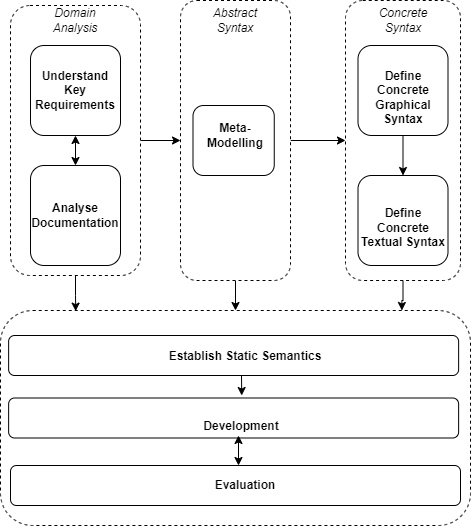
\includegraphics[width=0.5\textwidth]{diagrams/methods.png}
\label{methover}
\end{figure}

\subsection{Performing Domain Analysis}
Prior to developing formalisms for our language, we identified key concepts that are relevant to the domain in which our language would be used i.e. variability management in the robotics. We also identified and clarified the purpose of our language as well as the stakeholders our language is targetting. Finally, we identified all the relations between our gathered domain concepts which we derived from  from both stakeholders and relevant documentation, by studying the properties of our domain concepts.
\subsection{Implementation}
In our language implementation step, we define the capabilities of our language based on prior knowledge from our domain analysis and then conceived both the both graphical and textual forms our language, to represent the syntactic structure of our language tokens. Graphically, we used feature models to define and model features of robot examples. On an abstract level, we used class diagrams to model the capabilities present in our language.

\subsubsection{Defining the Abstract Syntax}
In creating the abstract syntax of our language, we formalised prior knowledge gathered in our domain analysis step into models. These models, otherwise known as meta-models were then refined in multiple iterations to reflect the requirements that form the capabilities of our variability-modelling language with respect to the problem space. We followed the following concrete steps to realise the abstract syntax of our language.\begin{enumerate*}
    \item Create a single decomposition of a class diagram together with compositional relationships.
    \item Verify the manner in which concepts are classified, and classes are organized in a hierarchy.
    \item Concretize relationships if need be. If relationships between concepts posses properties, they need to be transformed into classes.
    \item Remove redundancies by finding and removing multiple classes that have the same property.
    \item Evaluate resultant abstract syntax based on how accurately it reflects the problem and how well the concepts of design were kept within scope.
\end{enumerate*}

\subsubsection{Defining the Concrete Syntax}
The concrete syntax of our language is expressed both graphically and textually through feature models and JSON notation respectively. A major requirement of our implementation is to give potential users the expressive capability to create their own custom programs that will be in the form of robotic models. In that, end users of our domain specific language have the ability to implement their own feature models of example robots that are adaptable in varying contexts. In a graphical context, feature models of example systems were conceptualised and implemented with FeatureIDE\foot{https://featureide.github.io/} and then further translated into JSON notation made up of multiple intuitive and configurable attributes.

\subsection{Establishing the Static Semantics}
After defining both the concrete and abstract syntax of our language, we proceeded to establish the static semantics of our language. The static semantics in this context, refers to the underlying rules that determine the validity of models and configurations that can be created with our language. Key aspects of the static semantics which we clarified and established include:
\begin{enumerate}
    \item Outlining mechanisms that realise static and dynamic binding.
    \item Describing the configuration space that defines the configurability of our model instances.
    \item Constraining the configuration space.
\end{enumerate}

\subsection{Development}
In the development phase of our methodology, we utilised domain knowledge gathered from our domain analysis, concrete syntax definition, abstract syntax definition and static semantics as input to implement our domain specific language as a Python library. Our development approach can be summarized in the following steps:
\begin{enumerate}
    \item Gather system requirements by establishing the purpose of the language with regards to its functionality.
    \item Analyse requirements by transforming its specified textual functionalities into concrete functional and non-functional requirements.
    \item Establish design decisions such as the general architecture of the system, dependency management, choice of technologies and trade-offs, as well as implementation algorithms.
    \item Realise designs with algorithms and data structures from Python. However, given the fact that this is a language agnostic solution, even though majority of the implementation was in Python, there were still some minor C++\foot{https://isocpp.org/} implementations.
    \item Test system functionalities with both exploratory and unit tests by verifying test results against expected outputs.
 \end{enumerate}
 
\subsection{Language Evaluation Overview}
Evaluating our library means to assess our implementation from three main perspectives. These perspectives include \begin{enumerate*}[label=(\roman*)]
\item Correctness,
\item Realizability and
\item Novelty.
\end{enumerate*}
\begin{itemize}
    \item \textbf{Correctness:} The validity of models and configurations created with our language alongside the implied effect of feature constraints is closely evaluated by both a schema checker and a constraint checker's ability to detect syntax and constraint violations and prompt the end user accordingly.
    
    \item \textbf{Realizability:} Proof of realizability indicates that our binding technique which forms the core of our implemented variability mechanisms is feasible.
    
    \item \textbf{Novelty:} The novelty of our work is assessed along the lines of the innovative and conceptual uniqueness that defines the binding technique of our variability mechanism.
\end{itemize}

By realising our variability modelling language to implement binding time and binding mode mechanisms in a manner that fulfils our research objectives, we have automatically provided evidence that can be used to evaluate the realizability and novelty of our binding technique. In addition to this, we implemented a comprehensive evaluation plans to test for type and syntax correctness.

\subsection{Correctness Evaluation}
As a functional requirement of our language, end users have the ability to model robotic features, define configurations for each feature, and then apply such configurations to multiple scenarios. Configurations are typically an amalgamation of features, relationships and constraints. To assess the validity of configurations described with our language, we have implemented mechanisms that can be used to evaluate such user defined configurations. On a high level, our evaluation plan for our modelling language can be summarised as follows:
\begin{enumerate}
  \item Realise a mock-up of an example robotic system.
  \item Define binding configurations for each mock-up example.
  \item Plug in source code implementations of defined mock-up features.
  \item Compile and validate model and configuration syntax and semantics.
  \item Execute and test the model variability.
\end{enumerate}
For stakeholders such as end users to be able to verify the correctness of their models, all models defined in our modelling language must be validated on multiple levels of correctness i.e. syntax and semantic correctness. 
\begin{itemize}[label={}]
  \item \textbf{Syntax Validation: }To effectively validate the syntax of our language, we validate the schema of both model objects and configuration objects. Schema validation in this sense refers to token and token state validation.
 
  \item \textbf{Semantics Validation: } To validate the semantic implications of our language, we evaluate the correctness of configuration bindings in relation to the corresponding binding constraints specified. We also evaluate the correctness of each configuration binding pair with respect to its implied effect on other features in a given configuration space.
  
\end{itemize}


\section{Results}
\subsection{Architectural Overview}
Architecturally, our language consists of three modular components. These components include a syntax manager, a configuration manager, a source code implementation manager. As shown in figure \ref{arch-over} all these components are encapsulated and offered as a ROS compatible library.

The syntax manager component embodies the tokens as well as the lexical and syntactical schemas of our language. Tokens indicate the legal keywords or lexemes that are permissible in our language. There are two schema representations present in our language i.e. the feature schema and the configuration schema. Language schemas are simply represented as an object of tokens mapped to selected data structures. Listing \ref{feat-schema} and \ref{bind-schema} show samples of a feature schema and a configuration schema respectively.

\begin{listing}
\caption{Feature Schema}
\begin{minted}[
framesep=2mm,
baselinestretch=1.2,
bgcolor=LightGray,
fontsize=\footnotesize
]{Json}

    {
        "id": "F0",
        "name": "ComponentControl",
            "constraints": {
            "featuresIncluded": [],
            "featuresExcluded": [],
            "bindingTimeAllowed":"Early",
            "bindingModeAllowed":"Static"
            },
        "group": "OR",
        "isMandatory": true
    }

\end{minted}
\label{feat-schema}
\end{listing}

\begin{listing}
\caption{Configuration Schema}
\begin{minted}[
framesep=2mm,
baselinestretch=1.2,
bgcolor=LightGray,
fontsize=\footnotesize
]{Json}

{
    "id": "F0",
    "props": {
        "mode": "Static",
        "time": "Early"
    }
}
\end{minted}
\label{bind-schema}
\end{listing}

The configuration manager component of our library is made up of two parts. Namely, a binding semantics interpreter and a constraint checker. In general, variability management provides two main capabilities i.e. feature modelling and variation point definition and management. The binding semantics interpreter assimilates and displays the result of the interaction between the binding pairs of any pair of features. The constraint checker on the other hand parses the entire model definition to evaluate it for constraint violations in an attempt to validate user defined configurations with respect to the configuration space. Thus, the constraint checker enforces configuration rules that define the adaptability of configurations based on feature binding time and binding mode.
The source code implementation manager encapsulates a plug-in management interface which provides an integration point where end users can include source code implementations of modelled features into their configurations.

\begin{figure}[H]
\caption{Architectural Overview of Variability Management Solution}
\centering
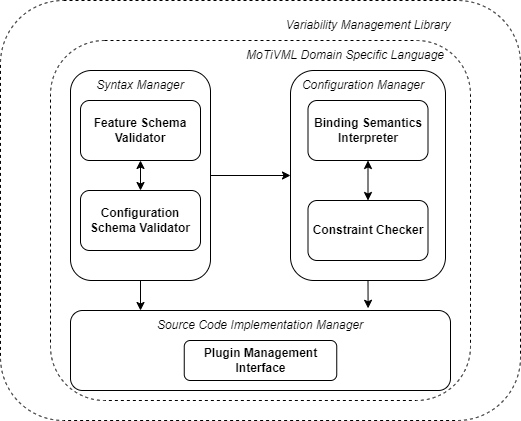
\includegraphics[width=0.5\textwidth]{diagrams/arch-overview.png}
\label{arch-over}
\end{figure}

\subsection{Domain Analysis}
In designing our language, we clarified the key relevant aspects of the domain in which our language will be used. We also identified key concepts and relationships that define the type of programs which domain stakeholders will be capable of writing with our language. The concepts we identified, together with their relationships were then formalized in the form of a model, and iteratively refined to describe the abstract syntax of our domain specific language as accurately as possible. 

During our domain analysis, we identified five standard questions which make up the core ideas and knowledge base upon which our language is built. 
    \begin{itemize}
        \item \textbf{Purpose: } \textit{What is the purpose of this language?}\\
        The purpose of our language is to provide roboticists with means and techniques for planning, designing, and implementing variability through mechanisms, that implement binding time and binding mode techniques.
        \item \textbf{Stakeholders: } \textit{Who are the key stakeholders and the intended users of the language?}\\ Our language targets a very diverse group of skilled professionals in the robotics domain who can be classified as end users. These stakeholders/end users include 
        \begin{enumerate*}[label=(\roman*)]
            \item Operators: End users with minimal training on the usage of our framework that the ability to operate robotic applications with pre-configured configurations.
            \item Developers: End users in charge of developing new features and implementing them into our framework.
            \item System Engineers: End users in charge of adapting the framework to the specific requirements of a customer.
        \end{enumerate*}
        \item \textbf{Concepts: }\textit{What are the key domain concepts that targetted stakeholders care about?}\\ From an end user perspective, concepts such as simplified feature modelling techniques, standardized configuration management techniques and flexible and customizable feature binding based on time and mode are key.
        \item \textbf{Relations: }\textit{How are domain concepts related, and what are their relevant properties?}\\
        Properties that define the core user concepts of our language include:
        \begin{itemize}
            \item Every instance of a feature class is selected by default.
            \item All features in a model are defined as mandatory by default upon instantiation.
            \item A parent feature may have zero or more child features.
            \item A modelled feature may have zero or more groups but a group must have two or more features to exist.
            \item A grouped set of features may belong to an OR or XOR group.
            \item A feature must have a binding time property which is set to \textit{Early} by default.
            \item A feature must have a binding mode property which is set to \textit{Static} by default.
            \item A modelled feature's binding time property can only exist in three states. i.e. \textit{Early, Late, Any}.
            \item A modelled feature's binding mode property can only exist in three states. i.e. \textit{Static, Dynamic, Any}.
        \end{itemize}
        \item \textbf{Examples: }\textit{What examples of language instances are available?}\\
        To the best of our knowledge, no language designed to model variability in robotic systems using binding time and binding mode exists. Our language is built on novel principles crafted to effectively manage variability in ROS based robotic systems.
    \end{itemize}
    
\subsection{Implementation}
In our implemented architecture, configuration capabilities are decoupled from feature capabilities. This is to primarily separate concerns by detaching feature attributes that do not require end user manipulation to form configurations from the ones that actually require it. Each set of decoupled configuration attributes references a corresponding feature by an \textit{ID} attribute.

\subsubsection{Developing Mock-up Examples}
An important use case of our language is that, it can be used to develop mock up examples that demonstrate the language's expressiveness. In the context of our study, examples refer to modelled features of robot product lines. Figure \ref{ex1} and \ref{ex2} show graphical representations in the form of feature models, of our selected example systems i.e. service robots. For each feature present in a model, we can express it textually with tokens from our language as shown in Figure \ref{feat-conc-text} and \ref{bind-conc-text}. Inspiration for these examples were drawn from general utility robots and disinfection robot product lines such as TIAGo and UVD Model C.
    
\begin{figure}[H]
\caption{Modelled Example One}
\centering
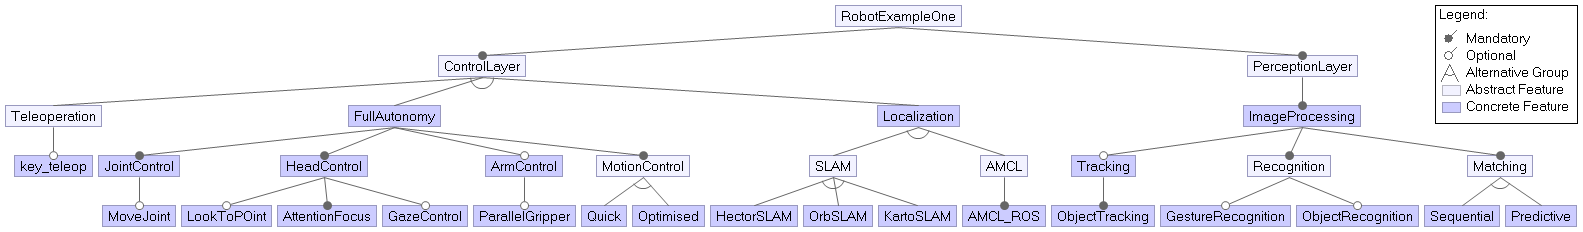
\includegraphics[width=\columnwidth]{diagrams/ex1.png}
\label{ex1}
\end{figure}

\begin{figure}[H]
\caption{Modelled Example Two}
\centering
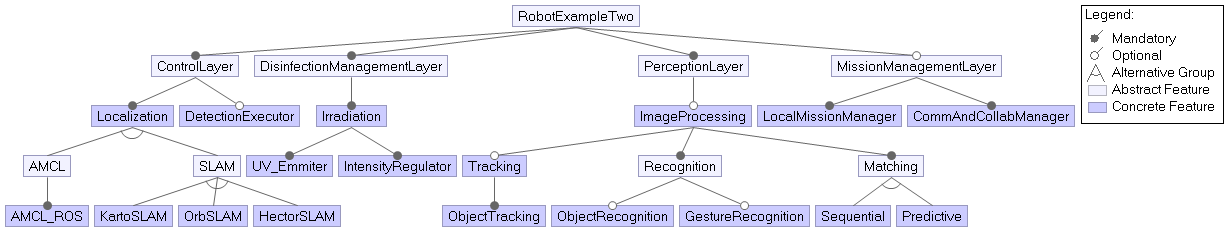
\includegraphics[width=\columnwidth]{diagrams/ex2.png}
\label{ex2}
\end{figure}
    
Furthermore, in our model refinement step, that aims at extending our mock-up examples against our requirements, we analyse the requirements associated with our language, justify if these requirements are met and then proceed to provide examples or evidence of said requirements that have been fulfilled.

\begin{listing}
\caption{Textual Sample of Features}
\begin{minted}[
framesep=2mm,
baselinestretch=1.2,
bgcolor=LightGray,
fontsize=\footnotesize
]{Json}
{
    "id": "root_feature",
    "name": "simpleBot",
    "group": "",
    "isMandatory": true,
    "sub": [
        {
        "id": "F0",
        "name": "ComponentControl",
        "constraints": {
        "featuresIncluded": [],
        "featuresExcluded": [],
        "bindingTimeAllowed":"Early",
        "bindingModeAllowed":"Static"
        },
        "group": "OR",
        "isMandatory": true
        "sub":[
            {
            "id": "F1",
            "name": "Localization",
            "constraints": {
            "featuresIncluded": [],
            "featuresExcluded": [],
            "bindingTimeAllowed":"Early",
            "bindingModeAllowed":"Static"
            },
            "group": "",
            "isMandatory": true
            }]}]}
\end{minted}
\label{feat-conc-text}
\end{listing}

All features present in our feature model specification posses binding time and binding mode configurations which can be used by our language to manage variability within a modelled robotic system. As indicated in our architectural design, configuration attributes are separated from feature attributes for the sole purpose of creating a clear distinction between configurable and no-configurable attributes. Listing
\ref{bind-conc-text} captures a sample representation of the concrete textual syntax of a feature's configuration attributes.

\begin{listing}
\caption{Textual Sample of Feature Bindings}
\begin{minted}[
framesep=2mm,
baselinestretch=1.2,
bgcolor=LightGray,
fontsize=\footnotesize
]{Json}
{
"properties": [
    {
    "id": "F0",
    "props": {
        "mode": "Static",
        "time": "Early"
    }
    },
    {
    "id": "F1",
    "props": {
        "mode": "Static",
        "time": "Early"
    }
    }
]
}
\end{minted}
\label{bind-conc-text}
\end{listing}

\subsubsection{Extending Mock-up Examples Against Requirements}
In our domain analysis we were able to understand key requirements relevant to our language implementation. Based on this understanding, we extended our mock up example in Figure \ref{ex1} and \ref{ex2} against our already established language requirements. Established language requirements include:
\begin{enumerate}
    \item R1: End users can instantiate robotic models
    \item R2: End users can create instances of features within models
    \item R3: End users can create decoupled model configurations
    \item R4: End users can create and link configurations to feature instances
    \item R5: End users can evaluate models both syntactically and semantically
\end{enumerate}
Using the concrete textual syntax of our modelling language which we have highlighted in Listing \ref{feat-conc-text} and \ref{bind-conc-text}, we identified example syntax representations that fulfil all the requirements listed above. Table \ref{tab:reqext} captures a mapping of each requirement along with its example syntax representation, that justifies that a requirement has been fulfilled.

\begin{table}[htbp]
\caption{Extended Mock-up Examples Against Requirements}
\begin{center}
\begin{tabular}{|c|c|}
\hline
    Requirement & Example Syntax  \\ \hline
     R1 & \multirow{2}{*}{$\{"id":"root\_feature","name":"simpleBot",$}\\
                        & \\
                        & $"group": "","isMandatory": true,"sub": []\}$\\ \hline
     R2 & \multirow{2}{*}{$\{"id": "F1","name": "Localization",$}\\ 
                        & \\
                        & $"constraints": \{"featuresIncluded": [],$\\ 
                        & $"featuresExcluded": [],$\\
                        &$"bindingTimeAllowed":"Early",$ \\
                        & $"bindingModeAllowed":"Static"\},$\\ 
                        & $"group": "","isMandatory": true\}$ \\
                         \hline
     R3 &  \multirow{2}{*}{$\{"id": "F1","props": \{$}\\
            & \\
            & $"mode": "Static","time": "Early"\}\}$\\
            & \\
            \hline
     R4 & $"props": \{"mode": "Static","time": "Early"\}\}$\\ \hline
     R5 & \multirow{2}{*}{Using the schema checker and constraint checker}\\ 
        & \\
        & model syntax, grammar and semantics can be evaluated\\ \hline
\end{tabular}
\label{tab:reqext}
\end{center}
\end{table}

\subsubsection{Identifying Language Tokens}
From a lexical standpoint, our language possesses a defined set of legal or permissible tokens. These tokens form part of a key-value pair production. Tokens can be identified and extracted from the key-value pair attributes that make up a feature in our language representation of a feature model. Table \ref{tab:langlex} shows all identified tokens together with their corresponding regular expressions that define their legal or valid lexical structures.

For each identified token in our language, we translated a valid expression of it into a regular expression to demonstrate which valid forms of these token can exist in our language. Syntactically, features and their configurations in our language model attributes as key value pairs wrapped in an object. Table \ref{tab:langlex} capture our list of identified tokens mapped to their corresponding regular expression formalisms.

\begin{table}[htbp]
\caption{Language Tokens}
\begin{center}
\begin{tabular}{|c|c|c|}
\hline
    Token & Regular Expression & Terminal Symbol \\\hline
                             id & 'id' & Id  \\\hline
                             name & 'name' & Name \\ \hline
                             featuresIncluded & 'featuresIncluded' & FeaturesIncluded\\ \hline
                             featuresExcluded & 'featuresExcluded' & FeaturesExcluded\\ \hline
                             bindingTimeAllowed & 'bindingTimeAllowed' & BindingTimeAllowed\\ \hline
                             bindingModeAllowed & 'bindingModeAllowed' & BindingModeAllowed\\\hline
                             group & 'group' & Group\\ \hline
                             isMandatory & 'isMandatory' & IsMandatory\\ \hline
                             time & 'time' & Time\\ \hline
                             mode & 'mode' & Mode\\ \hline
                              "Early" & 'Early' & Early\\ \hline
                              "Late" & 'Late' & Late\\ \hline
                              "Static" & 'Static' & Static\\ \hline
                              "Dynamic" & 'Dynamic' & Dynamic\\ \hline
                              "Any" & 'Any' & Any\\ \hline
                              "true" & 'true' & True\\ \hline
                              "false" & 'false' & False\\ \hline
                              "OR" & 'OR' & OR\\ \hline
                              "XOR" & 'XOR' & XOR\\ \hline
                              alphaValue & $(a-zA-Z)^+$ & alphaVal\\ \hline
                              alphanumValue & $(a-zA-Z0-9)^+$ & anumVal\\ \hline
                              boolValue & $[true | false]$ & boolVal\\ \hline
\end{tabular}
\label{tab:langlex}
\end{center}
\end{table}

\subsubsection{Specifying Language Terminals}
Considering the key-value paired nature of our language, its syntax can be described as a production consisting of a left-hand-side non-terminal, a colon (:) separator, followed by one or more right-hand-side sentences made up of varying forms of terminal and non-terminal symbols. Table \ref{tab:langlex} captures all terminal symbols present in our language.

\subsubsection{Identifying Syntactic Categories Within Our Language}
Our modelling language provides domain stakeholders with a means of instantiating a feature model, as well as the possibility of defining and configuring features. Within our language's concrete syntax, we can identify three distinct syntactic categories. These categories include:
\begin{enumerate}
    \item \textbf{featureDescriptionBlock:} This is made up of all feature attributes that are concerned with describing the general purpose of a feature. Although this category is not explicitly expressed in the textual formalism of a feature's schema, it can still be defined as a set of individual feature attributes which intuitively provide descriptive contexts to the functionality and purpose of a feature.
    \item \textbf{constraintsDefinitionBlock:} This is represented as a nested block of feature attributes that define the type constraints applicable to a feature as well as the set of possible constraint values that are valid for that feature.
    \item \textbf{bindingPropertiesBlock:} For every feature, there exists a corresponding configuration. Within the configuration of a feature exists a binding property block definition. The purpose of this binding property block is to allow domain stakeholders to configure binding time and binding mode attributes for each feature they define. These binding time and binding mode attribute definitions serve as the fundamental variation mechanism for each feature model.
\end{enumerate}
 
\subsubsection{Specifying Grammar Rules} By combining the terminals identified in Table \ref{tab:langlex} with the syntactic categories identified, we were able derive grammar productions for our language. The grammar rules for all three syntactic categories can be expressed as follows:\\

\begin{itemize}
	\item[] featureDescriptionBlock $\longrightarrow$ '\{'\ 'id'\ ':'\ anumVal,\ 'name'\ ':'\ alphaVal,\ 'group'\ ':'\ alphaVal, 'isMandatory'\ ':'\ boolVal\ '\}' \\
	
	\item[] constraintsDefinitionBlock $\longrightarrow$ constraints: '\{'\ 'featuresIncluded'\ ':'\ '['\ Id, Id, ...\ ']',\ 'featuresExcluded'\ ':'\ '['\ Id, Id, ...\ ']',\ 'bindingTimeAllowed'\ ':'\ alphaVal,\ 'bindingModeAllowed'\ ':'\ alphaVal '\}'\\
	
	\item[] bindingPropertiesBlock $\longrightarrow$ '\{'\ 'time'\ ':'\ alphaVal,\ 'mode'\ ':'\ alphaVal '\}'\\
\end{itemize}

\subsubsection{Abstract Syntax Definition}
The abstract syntax of any language refers to the logical representation of that language in memory. In figure \ref{femet} and \ref{conmet} we provide an abstraction to the user interfaces of both a feature and a configuration objects in the form of class diagrams. Upon instantiation, a feature is selected by default. A feature has the potential of having zero or more sub-features. Two or more sub-features may be grouped together in an OR or XOR group. Each feature's binding property constraint may be set to an \textit{ANY} value. This implies that a binding property may assume a value of either \textit{EARLY} or \textit{LATE} for binding time and \textit{STATIC} or \textit{DYNAMIC} for binding mode. Every existing feature in a model must bear a unique \textit{ID} attribute which serves as a reference point for each feature throughout multiple points in our implementation. A feature bears a \textit{NAME} that describes its capability. 

Furthermore, every feature has a set of constraints which define the scope of the feature in the model configuration space. Feature constraints are categorised into two main groups. i.e. cross functional constraints and binding property constraints.  Cross functional constraints refer to \textit{includes} and \textit{excludes} constraints while binding property constraints define the possible state values of binding time and binding mode attributes within configurations.

\begin{figure}[H]
\caption{Feature Meta Model}
\centering
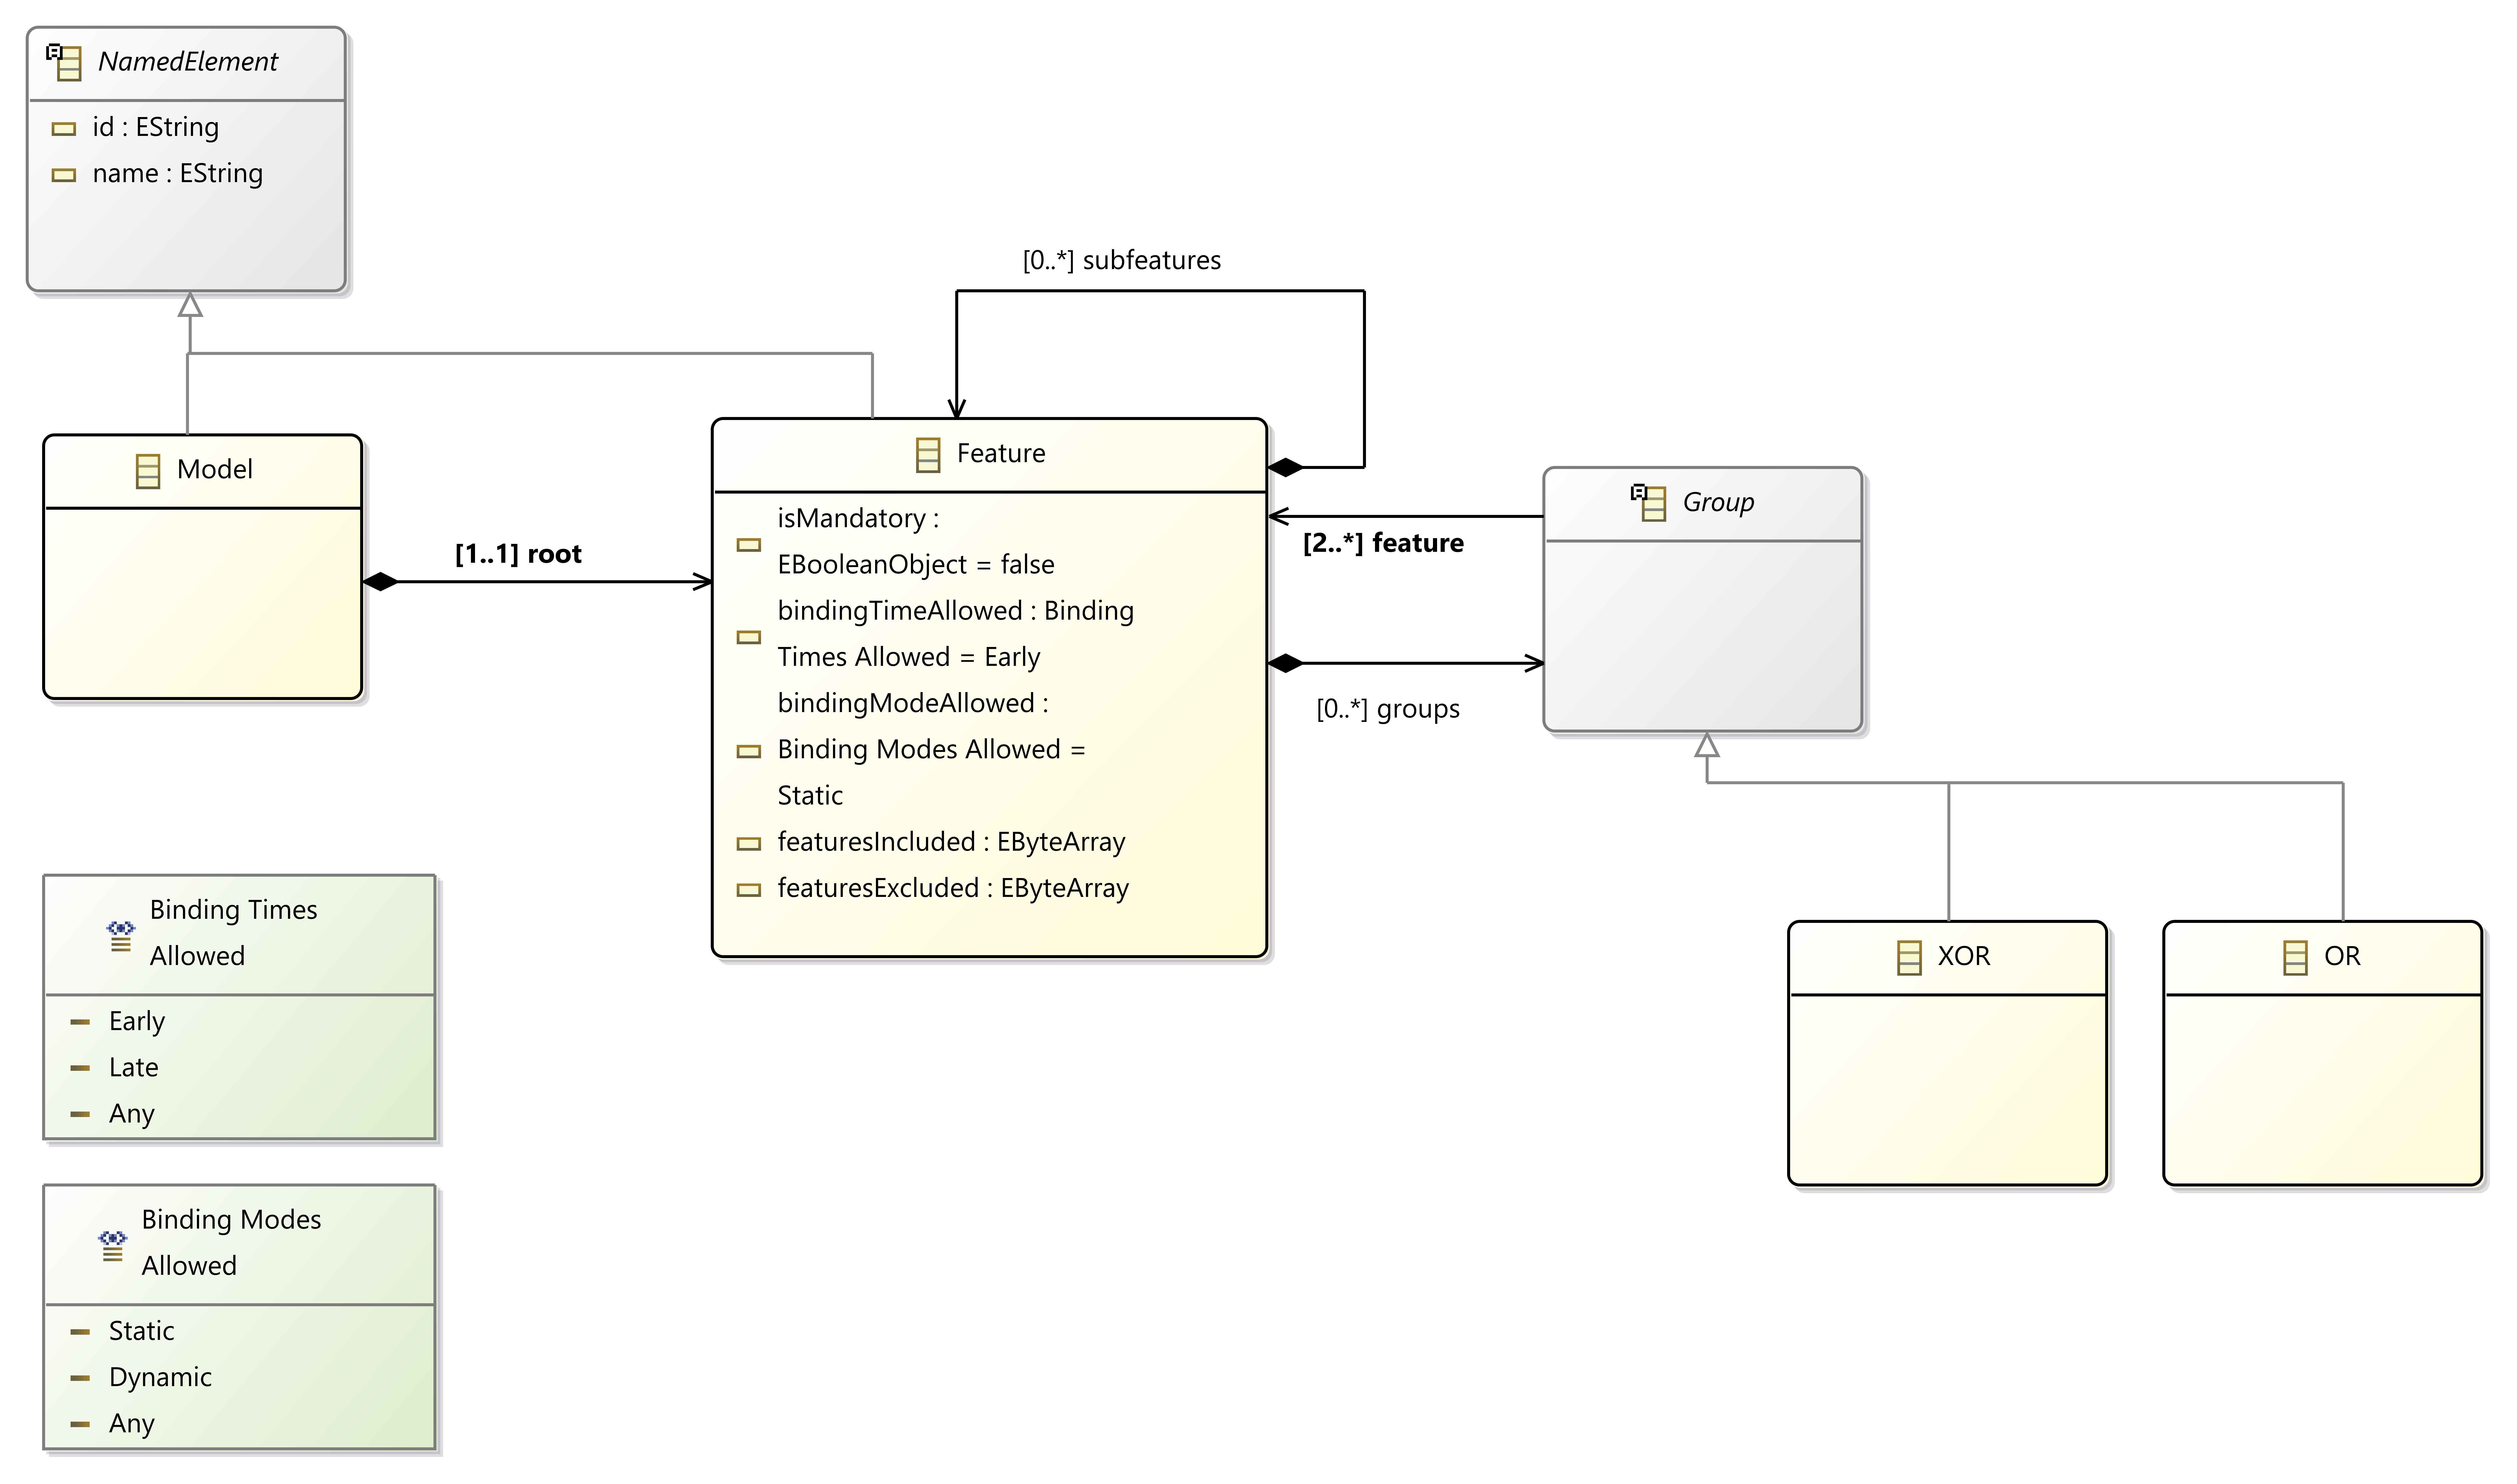
\includegraphics[width=0.5\textwidth]{diagrams/feature.png}
\label{femet}
\end{figure}

The configuration capabilities of a feature reflects the ability of the feature to be adapted to fit multiple contexts. Per our proposed variability management technique,
feature adaptations are determined by a binding time and binding mode combination, specified or assigned based on end user preferences. Each configuration bears reference to an existing feature by way of an \textit{ID} attribute. For each feature, there can exist multiple configurations, provided these configurations are valid with respect to the feature constraints.

\begin{figure}[H]
\caption{Configuration Meta Model}
\centering
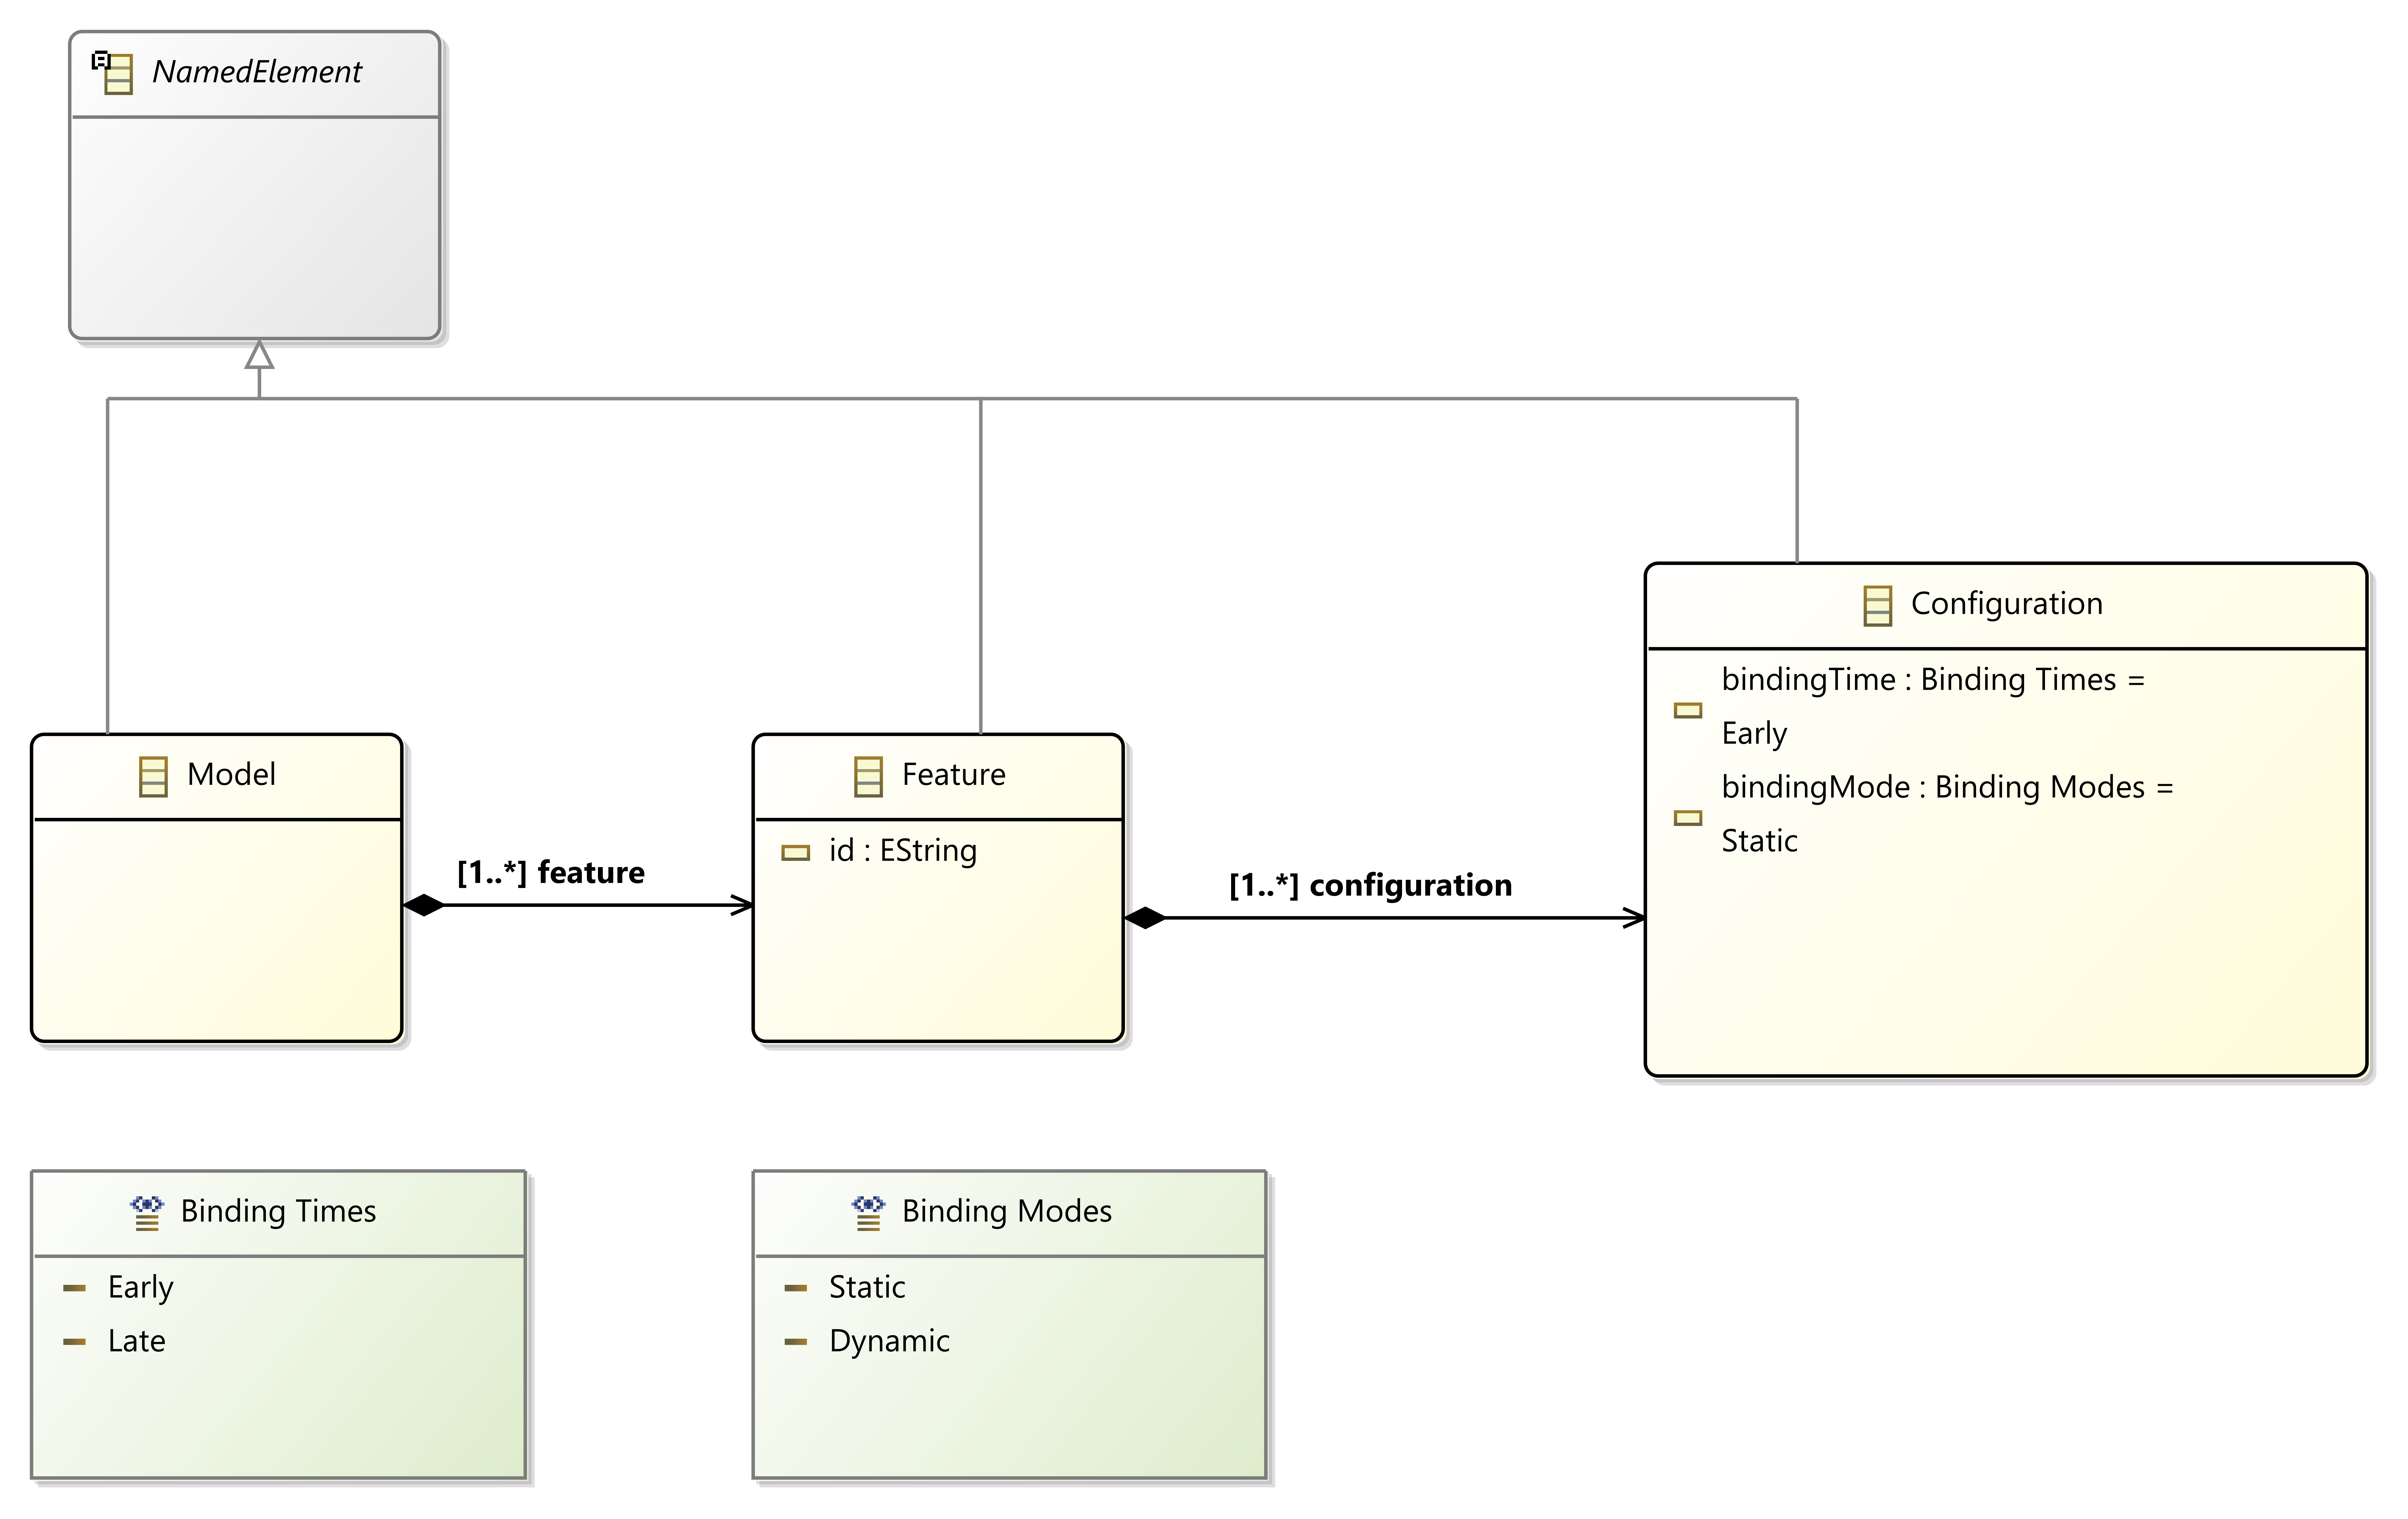
\includegraphics[width=0.5\textwidth]{diagrams/config.png}
\label{conmet}
\end{figure}

\subsubsection{Identifying Mechanisms That Realise Static and Dynamic Binding}
Realising static and dynamic binding in robotic applications can be tricky due to programming language compatibility and limitations. For both static and dynamic binding, there are both C++ and Python mechanisms that can be used to realise them as shown in Table \ref{tab:realmecha}. However, integrating both the C++ preprocessor and ROS pluginlib into implementations may not be feasible due to language compatibility issues. Thus, to realise static and dynamic binding in a ROS based application, various mechanisms can be leveraged upon. As indicated in Table \ref{tab:realmecha} below, the C preprocessor, antenna, rosrun and roalaunch can be used to implement static binding while ROS pluginlib and ROS parameters can be used to implement dynamic binding.

When it comes to time binding robotic features, again roslaunch and ROS parameters can be used to implement compile time binding, while ROS parameters can be used for runtime binding.

\begin{table}[htbp]
	\caption{Static and Dynamic Binding Mechanisms}
	\begin{center}
		\begin{tabular}{|c|c|}
			\hline
			Binding & Mechanisms  \\ \hline
			Static & C preprocessor, antenna, rosrun, roslaunch \\ \hline
			Dynamic &  ROS pluginlib, ROS parameters  \\ \hline
			Early &  roslaunch, ROS parameters  \\ \hline
			Late &  ROS parameters  \\ \hline
		\end{tabular}
		\label{tab:realmecha}
	\end{center}
\end{table}

\subsection{Static Semantics}
In the compile time state of our variability modelling language, program syntax is evaluated based on internally established feature relationships and constraints that define the static semantics of our language.

The scope of our static semantics, which can be verified  at compile time, includes data type evaluation i.e.  whether or not all tokens have been declared, which token declaration applies to which instances and so on. When it comes to controlling the semantic scope, constraint type declaration and implementation as well as the model level effect of constraints on each other can be inferred from feature interaction in a configuration.

\subsubsection{Describing the Configuration Space}
As shown in the concrete syntax of our feature modelling language, every instance of a feature has a binding time and binding mode attribute. The effect of the interaction between feature binding attributes has a major effect on the configuration space. In addition, each feature possess dependencies and constraints that validate defined feature instances. With the aid of propositional logic, table \ref{tab:propmap} provides an outlook into the configuration space of model instances. Per the results displayed in table \ref{tab:propmap}, mandatory features exhibit a bidirectional logical relationship between features indicating that both features require each other in all instances in which they are implemented. Conversely, an optional feature indicates a unidirectional behavior between a parent and child feature, where a child feature may imply a parent feature but the parent feature on the other hand can exist without that child feature. For cross-functional constraints such as includes and excludes, includes translates to an implication constraint while excludes could be represented as  A $\Rightarrow$ $\neg$ B \ or \ $\neg$ (A $\land$ B).

\begin{table}[htbp]
\caption{Propositional Logic Mapping for Feature Model Attributes}
\begin{center}
%\begin{tabular}{|c|c|c|}
\begin{tabular}{|P{2.5cm}|P{2.5cm}|P{2.5cm}|}
\hline
    Attribute Name & Feature Model Notation & Propositional Logic  \\ \hline
    Mandatory & 
\vspace{0.3px}    
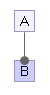
\includegraphics[width=10mm, height=12mm]{diagrams/mandatory.png} & A $ \Leftrightarrow $ B \\ \hline
    Optional &\vspace{0.3px} 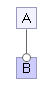
\includegraphics[width=10mm, height=12mm]{diagrams/optional.png}  & A $ \Rightarrow $ B \\ \hline
    Includes (requires) & A implies B &  A $ \Rightarrow $ B \\ \hline
    Excludes & A implies (Not B) &  A $ \Rightarrow $ $ \neg $ B \\ \hline
\end{tabular}
\label{tab:propmap}
\end{center}
\end{table}

The underlying logic of this language design requires the interaction of a feature's binding time and binding mode attributes, that serves as a variation mechanism for all feature models defined with this language. Table \ref{tab:timoconf} captures the semantics of possible binding time and binding mode combinations in any given model. This is relevant because, analysing the combined semantic effect of possible binding pairs in a model, gives insight into the feasibility or validity of combinations in the configuration space. Using propositional logic, Table \ref{tab:timoconf} shows the results of every possible interaction between binding pairs with respect to feature attributes such as mandatory, optional, includes and excludes. 

\begin{table}[H]
\caption{Feature Model Binding Semantics: \textbf{S = Static, E = Early, L = Late, D = Dynamic}}
\begin{center}
\begin{tabular}{|c|c|c|c|c|c|}
\hline
    A & B & B $ \Rightarrow $ A & A $ \Rightarrow $ B & A $ \Leftrightarrow $ B \\\hline
         SE & SE & 1 & 1 & 1  \\ \hline
         SE & SL & 1 & 0 & 0  \\ \hline
         SE & DE & 1 & 0 & 0 \\ \hline
         SE & DL & 1 & 0 & 0 \\ \hline
          
         SL & SL & 1 & 1 & 1 \\ \hline
         SL & DE & 0 & 0 & 0 \\ \hline
         SL & DL & 1 & 0 & 0 \\ \hline
         
         DE & DE & 0 & 0 & 0 \\ \hline
         DE & DL & 0 & 0 & 0 \\ \hline
         
         DL & DL & 0 & 0 & 0 \\ \hline
         
\end{tabular}
\label{tab:timoconf}
\end{center}
\end{table}

\subsubsection{Constraining the Configuration Space}
As part of our static semantics definition to effectively constrain the configuration space, it is relevant to enforce constraints on features. To do this, the following ground rules or pre-conditions were conceived as a fundamental basis for designing and developing our solution. We validate these constraints via an in-built constraint checker that parses configurations to identify constraint violations. The reasoning behind these constraints as well as their implied effects on configurations are discussed subsequently.
\begin{itemize}
    \item \textbf{Includes Constraint: }
    More often than not, some robotic features tend to require others to function. Supposing there are two features \textbf{A} and \textbf{B}, \textbf{A} \textit{includes} \textbf{B} would imply that, if feature \textbf{A} is selected, feature \textbf{B} must also be to be selected.
    %% give examples
    
    \item \textbf{Excludes Constraint: }
    Some robotic features on the other hand do not require others to function We express this as an excludes constraint in our implementation. Again, supposing there are two features \textbf{A} and \textbf{B}, \textbf{A} \textit{excludes} \textbf{B} would imply that when feature \textbf{A} is selected, feature \textbf{B} cannot be selected and vice versa.
    
    
    \item \textbf{Parent - Child Feature Constraint: }
    A static child feature cannot be a child of a dynamic parent. Allowing that form of inheritance would imply that an unloaded parent would create an orphan child feature. 
    

\item \textbf{Binding Property Constraints: }
As shown in our feature meta-model, the binding time and binding mode attributes of a feature are constrained to a set of valid inputs. By defining a set of valid binding time and mode input values, we are able to constrain the main feature attributes of user defined feature model instances.

\begin{table}[htbp]
\caption{Valid Binding Property Values}
\begin{center}
\begin{tabular}{|c|c|}
\hline
    Binding Property & Allowed State Values  \\ \hline
    Binding Time & Early, Late, Any \\ \hline
    Binding Mode & Static, Dynamic, Any\\ \hline
\end{tabular}
\label{tab:bpropcon}
\end{center}
\end{table}

\begin{itemize}
    \item \textbf{Binding Time:} The binding time attribute of a feature can assume three distinct values. Binding times can be set to \textit{early}, \textit{late} or \textit{any}. This means that features can either be strictly bound at compile time, strictly bound at runtime or can alternate between compile time and runtime state values.
    
    \item \textbf{Binding Mode:} The binding mode attribute of a feature can assume three distinct values as well. It can either have a \textit{static}, \textit{dynamic} or an \textit{any} value. This implies that a feature can either be strictly static, strictly dynamic or in the case of an \textit{any}, a feature can alternate between static and dynamic mode states.
\end{itemize}

\end{itemize}

\subsection{Implementing Defined Features}
As an extension to our modelling language, users do not only have the capability of defining and modelling features, but also have the capability of integrating source code implementations of features into their models. Through a language-agnostic interface, extracted source code implementations of features can be encapsulated and integrated into our library, where they can be referenced based on mechanisms provided within our implementation.

\section{Validation}
For us to be able to thoroughly validate our language design and its implementation, we have to ensure that we are able to evaluate user generated artifacts realised with our variability modelling language. These artifacts can be identified as feature models and configurations. In doing so, we translated graphical representations of our mock-up examples in Figure \ref{ex1} and \ref{ex2} into model and configuration instances of our language. We then went on to validate the models and configurations for syntax and semantic correctness. Validation mechanisms used for syntax and semantic validation include a schema checker and a constraint checker. The schema checker is used to evaluate the schema of all modelled features and configurations, whereas a constraint checker handles the semantic evaluation of bindings defined within our mock-up examples.

  \subsection{Schema Checker} Our library provides a schema checker which serves the purpose of validating the grammar and syntax rules of programs created with our language. Using our language, features and configurations can be modelled as key value pairs of objects. From a grammatical perspective, object keys are represented as tokens that are terminal in nature. Value tokens on the other hand are generated from a finite set of data types which are unique to each object attribute.
  
  The operations of our schema checker can be classified into two categories. i.e. validating the feature schema and validating the configuration schema. Feature schema validation involves validating a feature definition for valid id, name, constraints, group and optional status tokens in a feature definition. The absence or misrepresentation of any of such tokens triggers an error which is translated into a console prompt.
  
  \subsection{Constraint Checker} Embedded within our library is another component referred to as the constraint checker. This component purposefully evaluates the semantic implications of each feature's constraints against its configuration settings, in the configuration space. Our constraint checker component operates by parsing feature models to validate two main types of semantics. The first is the set of configurations that have been defined within the scope of the constraints enforced. And the second is the validity of configuration binding pairs with respect to other binding pairs within a specific product line definition.
  
  This capability of our library, backs the claim that our binding technique is flexible and customizable. An as such can be used to adapt product lines to fit varying usage contexts.


By evaluating our variability modelling language with respect to the challenges and the research questions we have previously highlighted in Section \ref{section:intro}, we can therefore assess the degree to which domain challenges that have driven this study have been fulfilled. In doing so, we analyse each domain challenge in close alignment with our research goals.

\subsection{Lack of a Flexible and Customizable Variability Modelling Language}
This challenge is addressed by the core mechanism that defines variation point implementation in our language. In our light-weight architecture, features in a model can be loaded and unloaded based on their binding times and binding modes. Architecturally, both features and configurations are modelled separately with the intention of simplifying the modelling experience by decoupling configurations from features. This decoupled nature of models reduces complexity by separating concerns.

Secondly, our variability modelling language is a ROS specific solution. In that, the entire language implementation is ROS dependent. The advantage here lies in ROS's set of software libraries and tools that provide a robust abstraction when building robotic applications. ROS ships with drivers, state-of-the-art algorithms and powerful developer tools that supports quick development and maintenance of robotic applications. Thus providing a standardised platform for our variability modelling language to be built upon.

The solution to this challenge ties directly into \textit{RQ 2} in Section \ref{section:intro} which asks the question of how a variability modelling language that allows features to be modelled together with their bindings can be designed. Where binding time and binding mode modelling guarantees flexibility and customizability in robotic system designs.

Furthermore, our library design targets a wide array of skilled professionals in the robotics domain. In this study, we take into consideration varying levels of skilled professionals from multiple backgrounds in the robotics domain. By so doing we are able to conceptualise and implement a language that meets the needs of domain stakeholders with different level of know-how.

\subsection{The lack of mechanisms and guidelines for implementing variability management techniques in robotic systems}
There have been some propositions in the area of managing variability in the robotics systems but none of them offer mechanisms and operational guidelines to assist domain stakeholders in understanding and using such languages. This scarcity is particularly prevalent in the ROS community. For this reason, more often than not, variability management is handled in an adhoc manner by experts in the robotics domain.

To alleviate this lack, our variability modelling library ships with a comprehensive set of guidelines\foot{https://github.com/SergioGarG/sera-extension/tree/master/documents/guidelineDoc/main.pdf}
offered as a supporting artifact that serves as verification for our variability modelling language. In this documentation, we verify that our language fulfils the requirements stated in our implementation, while providing demonstrated examples to prove it.

We deem guideline documentations as an integral part of robotics application development, for three main reasons. Namely, for the seamless advancement of robotic application development, to encourage the standard practice of building and maintaining open source robot applications and last but not least, to encourage transparency and reproducibility of relevant and useful robotic applications. Currently, this is lacking amongst open sourced robotic applications. Thus, in addition to this seminal study, we offer such a guideline document.

In addition to this, we have also identified and implemented mechanisms in this study, that can be used to model variability in any robotic system.

To verify the relevance of our language implementation guidelines and mechanisms, we realised mock up example of robots with feature instances that possess different binding times and binding modes to demonstrate the simple, lightweight and easy to understand nature of our variability modelling language as well as the underlying mechanisms which are capable of supporting variability modelling and management.

\subsection{Complexity of Engineering Robotic Systems}
Robotic systems are complex systems made up of complex applications integrated into one unified solution. Going by this premise, we can infer that the more a robotic system grows in functionality, the more the complexity of the system also grows. Modelling a complex system requires a modelling language that is both syntactically and semantically intuitive. Such a modelling language needs to be able to abstract irrelevant details from end users.

For this reason, in our modelling language, users have the capability of implementing features with different binding times and binding modes through mechanisms and guidelines that we have provided in our language (\textit{RQ 3}). Syntax representations in our concrete syntax design demonstrate a close mapping of user requirements with our language syntax. Likewise, on a semantic level, through our abstract syntax representations, the configuration space can be understood in terms of configuration interactions in model definitions.

Finally, all the above mentioned syntax and semantic architectural designs can be verified through in-built mechanisms that validate model implementations on a syntax and semantic level. These mechanisms namely, a schema checker and a constraint checker are designed to abstract the complexity of designing valid models by parsing and validating model definitions for correctness. 

\section*{Acknowledgment}
This journal draws inspiration from materials contributed by Sergio Garc\'{i}a, Claudio Menghi, Patrizio Pelliccione, Thorsten Berger and Rebekka Wohlrab. This study extends their work concerning SERA; A Self-adaptive dEcentralized Robotic Architecture for building autonomous, heterogeneous and collaborative robotic applications. 


\begin{thebibliography}{00}
\bibitem{sera} S. Garc\'{i}a, C. Menghi, P. Pelliccione, T. Berger, and R. Wohlrab, ``An Architecture for Decentralized, Collaborative, and Autonomous Robots,'' in Proceedings - 2018 IEEE 15th ICSA, 2018.
\bibitem{flex-feat-bind} M. Rosenmüller, N. Siegmund, S. Apel, and G. Saake, Flexible feature binding in Software Product Lines, Springer Science + Business Media, LLC 2011.
\bibitem{mb-approach} M. Wirkus, S. Arnold, E. Berghöfer, ``Online Reconfiguration of Distributed Robot Control Systems
for Modular Robot Behavior Implementation,'' in Journal of Intelligent \& Robotic Systems, Springer 2020.
\bibitem{feat-mod} D. Nešić, J. Krüger, Ş. Stănciulescu, T. Berger, ``Principles of Feature Modeling,'' in  Proceedings of the 2019 27th ACM Joint Meeting on European Software Engineering Conference and Symposium on the Foundations of Software Engineering, 2019.
\bibitem{feats} T. Berger, D. Lettner, J. Rubin, P. Grünbacher, A. Silva, M. Becker,  M. Chechik, K. Czarnecki, ``What is a Feature? A Qualitative Study of Features in Industrial Software Product Lines,'' in  Proceedings of the 19th International Conference on Software Product Line, 2015.
\bibitem{sparc} The Partnership for Robotics in Europe, ``Robotics 2020 Multi-Annual Roadmap For Robotics in Europe,'' in  Horizon 2020 Call ICT-2016 (ICT-25 \& ICT-26), 2020.
\bibitem{sple} K. Pohl, G. Böckler, F. van der Linden, ``Software Product Line Engineering Foundations, Principles, and Techniques,'' Springer, 2005.
\bibitem{variab} F. Bachmann, P. C. Clements, ``Variability in Software Product Lines,'' CMU/SEI, 2005.
\bibitem{robo-se} S. Garc\'{i}a, D. Strüber, P. Pelliccione, T. Berger, and D. Brugali, ``Robotics Software Engineering: A Perspective from the Service
Robotics Domain,''  ESEC/FSE, 2020.
\bibitem{des-res} A. R. Hevner, S. T. March, J. Park, S. Ram, ``Design Science In Information Systems Research,'' MIS Quarterly Vol. 28 No. 1, pp. 75-105, 2004.
\bibitem{serv-rob-his} M. Ceccarelli, ``Service Robots and Robotics: Design and Application,'' SCOPUS, 2012.
\bibitem{soft-arch-robo} A. Ahmad, M. A. Babar, ``Software architectures for robotic systems: A systematic mapping
study,'' The Journal of Systems and Software, 2016.
\bibitem{fmod-lang-scenarios} T. Berger, P. Collet, ``Usage Scenarios for a Common Feature Modeling Language,'' Association for Computing Machinery, 2019.
\bibitem{clafer} P. Juodisius, A. Sarkar, R. R. Mukkamala, M. Antkiewicz, K. Czarnecki, A. Wasowski, ``Clafer: Lightweight Modeling of Structure, Behaviour, and Variability,'' The Art, Science, and Engineering of Programming Journal, 2019.
\bibitem{mmrs} D. Bozhinoski, D. Garlan, I. Malavolta, P. Pelliccione, ``Managing safety and mission completion via collective run-time adaptation,'' Journal of Systems Architecture, 2019.
\bibitem{soft-arch} L. Bass, P. Clements, R. Kazman, ``Software Architecture in Practice, Third Edition,'' Addision-Wesley, 2013.
\bibitem{ref-arch} E. Y. Nakagawa, P. O. Antonino, M. Becker, ``Reference Architecture and Product Line Architecture: A Subtle But Critical Difference,'' 5th European conference on Software architecture (ECSA'11), 2011.
\bibitem{mod-driv-eng} D.C. Schmidt, ``Guest Editor's Introduction: Model-Driven Engineering,'' IEEE, 2006.
\bibitem{emb-sys}R. H. Bourgonjon, ``Embedded Systems in Consumer Products,'' Springer, Berlin, Heidelberg, 1995.
\bibitem{graph-mde} N. Hochgeschwender, S. Schneider, H. Voos, H. Bruyninckx, G. K. Kraetzschmar, ``Graph-based Software Knowledge: Storage and Semantic Querying of Domain Models for Run-Time Adaptation,'' iIEEE ICSE, Modeling, Berlin, Heidelberg, 2016.
\bibitem{model-centric} A. Steck, A. Lotz, C. Schlegel, ``Model-Driven Engineering and Run-Time Model-Usage in Service Robotics,'' ACM, 2011.
\bibitem{cont-aware} R. P. Pinto, E. Cardozo, P.R.S.L. Coelho, E. G. Guimarães, ``A Domain-independent Middleware Framework for Context-aware Applications,'' ACM/IFIP/USENIX International Middleware Conference, 2007.
\bibitem{var-mod-ind} T. Berger, R. Rublack, D. Nair, J. M. Atlee, M. Becker, K. Czarnecki, A. Wasowski, ``A Survey of Variability Modeling in Industrial Practice,'' University of Waterloo, 2013.
\bibitem{var-mech} T. Berger, R. Pfeiffer, R. Tartler, S. Dienst, K. Czarnecki, A. Wasowski,  S. She, ``Variability Mechanisms in Software Ecosystems,'' Chalmers University of Technology, 2014.
\bibitem{dsl} A. van Deursen, P. Klint, J. Visser, ``Domain-Specific Languages,'' ACM SIGPLAN Notices, 2000.
\bibitem{dy-sple} J. D. A. S. Eleutério, C. M. F. Rubira, ``A Comparative Study of Dynamic Software Product Line Solutions for Building Self-Adaptive Systems,'' Technical Report - IC-17-05 - Relatório Técnico, 2017.
\bibitem{s-adapt} M. Salehie, L. Tahvildari, ``Self-adaptive software: Landscape and Research Challenges,'' ACM Transactions on Autonomous and Adaptive Systems, 2009.
\bibitem{vsoft} M. Galster, P. Avgeriou, D. Weyns, T. Männistö, ``Variability in Software Architecture: Current Practice and Challenges,'' ACM SIGSOFT Software Engineering Notes, vol. 36, no. 5, pp. 30–32, 2011.
\bibitem{dsl-robo} A. Nordmann, N. Hochgeschwender, D. Wigand, and S. Wrede, ``A Survey on Domain-Specific Modeling and Languages in Robotics”, Journal of Software Engineering for Robotics,'' JOSER, 2016.
\bibitem{arch-prac} L. Bass, P. Clements, R. Kazman, ``Software Architecture in Practice,'' Third Edition Addison-Wesley, 2013.
\bibitem{com-stat-dy-bin} M. Rosenmüller, N. Siegmund, G. Saake, S. Apel, ``Combining Static and Dynamic Feature Binding in
Software Product Lines,'' Fakultät für InformatikOtto-von-Guericke-Universität Magdeburg, 2009.
\bibitem{tailor-spl} M. Rosenmüller, N. Siegmund, M. Pukall, S. Apel, ``Tailoring Dynamic Software Product Lines,'' GPCE, 2011.
\bibitem{lgherardi} L. Gherardi, ``Variability Modeling and Resolution in Component-based Robotics Systems,'' Thesis,  Universita degli Studi di Bergamo, 2013.
\bibitem{ros-ref} A. Koubaa, ``Robot Operating System (ROS), The Complete Reference (Volume 1),'' Springer, 2016.
\bibitem{pric-soft} T. Berger, A. Wasowski, ``Principles of Software Language Design,'' Chalmers $|$ University of Gothenburg, 2019.
\bibitem{handb} M. Ramachandran, R. Atem de Carvalho, ``Handbook of Research on Software Engineering and Productivity Technologies: Implications of Globalization,'' SCOPUS, 2009.
\bibitem{vmir} T. Berger, S. She, R. Lotufo, A. Wasowski, K. Czarnecki, ``Variability Modeling in the Real: A Perspective From the Operating Systems Domain,'' ACM, 2010.
\end{thebibliography}
\vspace{12pt}

\end{document}
